	% -----------------------------------------------
% Styl pro psaní diplomových a bakalářských prací
% Určeno pro překlad pdfcsLaTeXem
% -----------------------------------------------
\documentclass[a4paper,12pt]{book} % pro oboustranný tisk zvolte {book}!
% velikost stránky
\usepackage[tmargin=2cm,bmargin=2.5cm,rmargin=2cm,lmargin=3.5cm]{geometry}
% volba kódování, nastaveno je unicode
\usepackage[utf8]{inputenc}
% \usepackage[cp1250]{inputenc}
% \usepackage[latin2]{inputenc}
\usepackage[english]{babel}
%\def\refname{Literatura}
% pomocná makra pro sazbu matematických výrazů
\usepackage{amssymb} %na psaní dvojitých písem a zvlastních znaků (např. \varkappa)
\usepackage{amsmath}
% balíček pro vkládání obrázků
\usepackage{graphicx}
% balíček pro obrázky na krajích stránky 
%\usepackage{floatflt}
% balíček pro křížové odkazy
\usepackage[unicode,bookmarksopen,colorlinks=false,plainpages=false,urlcolor=blue,pdfpagelabels]{hyperref}
% balíček pro vkládání hypertextových odkazů
\usepackage{url}

\usepackage{float}


\usepackage[numbers]{natbib}

% -----------------------------------------------
% Přepínač mezi bakalářskou a diplomovou prací, 
% barevným a černobílým logem a mezi studentem a studentkou (vypracoval/vypracovala apod.)
% -----------------------------------------------
\newif\ifbakal\bakaltrue
\newif\ifbarva\barvafalse
\newif\ifstudentka\studentkafalse

% -----------------------------------------------
% Údaje o práci – doplní se i do bibliografické identifikace, pouze v prohlášení je nutné vložit jméno vedoucího práce, které není v 1. pádě
% -----------------------------------------------
\newcommand{\nazevcz}{Kalibrace a monitorování astročásticových teleskopů}
\newcommand{\nazev}{Calibration and monitoring of astroparticle telescopes}
\newcommand{\student}{Daniel Staník}
\ifbakal%
  \newcommand{\program}{B0533A110007  Applied Physics}%
  \newcommand{\obor}{1702R001  Applied Physics  (AFYZ)}%
  %\else%
  %\newcommand{\program}{N1701 Fyzika}%
  %\newcommand{\obor}{7504T055 Učitelství fyziky pro střední školy}%
\fi
\newcommand{\rokod}{2022}
\newcommand{\vedouci}{Ing. Ladislav Chytka, Ph.D.}
\newcommand{\abstrakt}{%
Lorem ipsum dolor sit amet, consectetur adipiscing elit. Curabitur et lectus sit amet lectus vestibulum dignissim. Cras sit amet enim vitae mi elementum blandit eget nec tortor. Curabitur eget eros vitae arcu luctus varius commodo vel mauris. Nam elementum convallis pretium. Nunc dignissim pulvinar urna, nec blandit ante fringilla at. Ut et magna purus, vel pellentesque massa. In tortor nisi, faucibus condimentum cursus ut, sollicitudin quis leo. Ut at purus nec arcu accumsan tincidunt id id massa. Nam id vehicula mi.}
% -----------------------------------------------
\newcommand{\abstrakten}{%
Lorem ipsum dolor sit amet, consectetur adipiscing elit. Curabitur et lectus sit amet lectus vestibulum dignissim. Cras sit amet enim vitae mi elementum blandit eget nec tortor. Curabitur eget eros vitae arcu luctus varius commodo vel mauris. Nam elementum convallis pretium. Nunc dignissim pulvinar urna, nec blandit ante fringilla at. Ut et magna purus, vel pellentesque massa. In tortor nisi, faucibus condimentum cursus ut, sollicitudin quis leo. Ut at purus nec arcu accumsan tincidunt id id massa. Nam id vehicula mi.}
% klíčová slova
\newcommand{\klic}{klíčové slovo 1, klíčové slovo 2, \ldots}
\newcommand{\klicen}{keyword 1, keyword 2, \ldots}
\newcommand{\pocetstran}{xx}
\newcommand{\pocetpriloh}{x}

% -----------------------------------------------
% Definice vlastních maker pro usnadnění psaní
% a opakování symbolů při zlomu řádku
% -----------------------------------------------
% implikace se opakuje
\def\Plyne{\Rightarrow\discretionary{}{\hbox{$\Rightarrow$}}{}}
% -----------------------------------------------
% ekvivalence se opakuje
\def\Ekviv{\Leftrightarrow\discretionary{}{\hbox{$\Leftrightarrow$}}{}}
% -----------------------------------------------
% % plus '+' se opakuje při zalomení řádku
\mathchardef\plus="202B
\mathcode`\+="8000
{\catcode`\+=\active
\gdef+{\plus\nobreak\discretionary{}{\hbox{$\plus$}}{}}}
% opakování - při zalomení řádku
\newsavebox{\minusbox}
\savebox{\minusbox}{\hbox{$-$}}
\def\aktivniminus #1{{\catcode`#1=13 \bgroup \uccode`~=`#1
\uppercase{\egroup\gdef~}{\mathminus\discretionary{}{\copy\minusbox}{}}}}
% % -----------------------------------------------
% % rovnitko '=' se opakuje
\def\aktivnirovnitko #1{{\catcode`#1=13 \bgroup \uccode`~=`#1
\uppercase{\egroup\gdef~}{\mathequal\discretionary{}{=}{}}}}
% -----------------------------------------------
% zrušení mezery za čárkou v matematickém reľimu
\mathcode`,="002C

% -----------------------------------------------
% Úprava matematické sazby
% -----------------------------------------------
\def\sgn{\mathop{\rm sgn}\nolimits}
\def\tg{\mathop{\rm tg}\nolimits}
\def\cotg{\mathop{\rm cotg}\nolimits}
\def\arctg{\mathop{\rm arctg}\nolimits}
% -----------------------------------------------
% vektory polotučným skloněným písmem
\DeclareFontFamily{OT1}{bssbf}{}
\DeclareFontShape{OT1}{bssbf}{m}{n}{<5> <6> <7> <8> <9> <10> <11> <12> <14.4> <17> <20> <20.74> <25> bssb10}{}
\newcommand{\vek}{\fontencoding{OT1}\fontfamily{bssbf}\selectfont}
\renewcommand{\vec}[1]{\hbox{\vek #1}\hspace*{1.5pt}}
% polotučná řecká písmena
\def\bgomega{\vec{\char151}}
     \def\bgOmega{\vec{\char10}}
     \def\bggamma{\vec{\char130}}
     \def\bgvarphi{\vec{\char161}}
     \def\bgphi{\vec{\char148}}
     \def\bgxi{\vec{\char142}}
     \def\bgtau{\vec{\char146}}
     \def\bgeta{\vec{\char134}}
     \def\bgmu{\vec{\char139}}
     \def\bgnu{\vec{\char140}}
     \def\bvarrho{\vec{\char157}}
     \def\bgsigma{\vec{\char145}}
     \def\bgpsi{\vec{\char150}}
     \def\bgchi{\vec{\char149}}
     \def\bgvartheta{\vec{\char154}}

% ---------------------------------------------------------------
% Samotná práce
% ---------------------------------------------------------------
\begin{document}
% -----------------------------------------------
% Titulní strana
% -----------------------------------------------
\pagestyle{empty}
\setbox0=\hbox{\LARGE\scshape Joint Laboratory of Optics}
\centerline{\LARGE\scshape  Palacký University Olomouc}

\bigskip
\centerline{\LARGE\scshape Faculty of Science}
   
\bigskip
\centerline{\box0}
  
\vfill
\centerline{\LARGE\bfseries \ifbakal{BACHELOR}\else{DIPLOMOVÁ}\fi\ THESIS}

\bigskip
\begin{center}
{\huge\nazev}  


\vfill
\ifbarva
\includegraphics[height=3cm]{up_logo_color}\else%

\includegraphics[height=3cm]{up_logo_bw}\fi

\vfill

\noindent%
\begin{tabular}{ll}
Author\ifstudentka{a}\fi: & {\bfseries\student}\\
Study program: &\program\\
Field of study: &\obor\\
Form of study:& Full-time\\
Supervisor:& \vedouci\\
Deadline:& April~\rokod
\end{tabular}
\end{center}

% ---------------------------------------------------------------
% Prohlášení
% -----------------------------------------------
\newpage
\hbox{~}

\vfill

\begin{center}
{\bf DECLARATION}
\end{center}

\noindent
I hereby declare that I elaborated this bachelor thesis independently under the supervision 
of  Ing. Ladislav Chytka, Ph.D.,  using  only  information  sources  referred  in  the  Literature chapter. \\
{}\vspace{3ex}

\noindent
In~Olomouc~\today   \hfill\parbox[t]{6cm}{\centering\null\dotfill\\\student}

% -----------------------------------------------
% Bibliografická anotace
% -----------------------------------------------
\newpage
% Bibliografická identifikace
\section*{Bibliographical identification}

\begin{tabular}{lp{8cm}}
%-----------
% \multicolumn{2}{c}{\bfseries Bibliographical identification}\\[8mm]
%-----------
Autor's first name and surname & \student\\
%-----------
Title & \nazev\\
%-----------
Type of thesis & \ifbakal{Bachelor}\else{Master}\fi \\
%-----------
Department & Joint Laboratory of Optics \\
%-----------
Supervisor & \vedouci\\
%-----------
The year of presentation & \rokod \\
%-----------
Abstract & \abstrakten\\
%-----------
Keywords & \klicen\\
%-----------
Number of pages & \pocetstran\\
%-----------
Number of appendices &  \pocetpriloh\\
%-----------
Language & czech\\
%-----------
\end{tabular}

% -----------------------------------------------

\newpage
\section*{Bibliografická identifikace}

\begin{tabular}{lp{8.5cm}}
%-----------
% \multicolumn{2}{c}{\bfseries Bibliografická identifikace}\\[8mm]
%-----------
Jméno a příjmení autora & \student\\
%-----------
Název práce & \nazevcz \\
%-----------
Typ práce & \ifbakal{Bakalářská}\else{Diplomová}\fi \\
%-----------
Pracoviště & Společná Laboratoř Optiky \\
%-----------
Vedoucí práce & \vedouci\\
%-----------
Rok obhajoby práce & \rokod\\
%-----------
Abstrakt & \abstrakt\\
%-----------
Klíčová slova & \klic\\
%-----------
Počet stran & \pocetstran\\
%-----------
Počet příloh & \pocetpriloh\\
%-----------
Jazyk & český\\
%-----------
\end{tabular}
% %%%%%%%%%%%%%%%%%%%%%%%% End of file %%%%%%%%%%%%%%%%%%%%%%%%





%%%% Tady začínáme %%%%%%%%%%%%%%%%%%%%%%%%%%%%%%%%%%%%%%%%%%%%%%%%%%%%%%%%%%
\newpage
%%%%%%%%%%%%%%%%%%%%%%%%%%%%%%%%%%%%%%%%%%%%%%%%%%%%%%%%%%%%%%%%%%%%%%%%%%%%%
\widowpenalty =10000
\pagestyle{plain}
% -----------------------------------------------
% Obsah je generován automaticky, změny se projeví po 2 překladech
% -----------------------------------------------
\tableofcontents

% -----------------------------------------------
% Úvod
% -----------------------------------------------
\chapter*{Introduction}
\addcontentsline{toc}{chapter}{Introduction}

Lorem ipsum dolor sit amet, consectetur adipiscing elit. Curabitur et lectus sit amet lectus vestibulum dignissim. Cras sit amet enim vitae mi elementum blandit eget nec tortor. Curabitur eget eros vitae arcu luctus varius commodo vel mauris. Nam elementum convallis pretium. Nunc dignissim pulvinar urna, nec blandit ante fringilla at. Ut et magna purus, vel pellentesque massa. In tortor nisi, faucibus condimentum cursus ut, sollicitudin quis leo. Ut at purus nec arcu accumsan tincidunt id id massa. Nam id vehicula mi. 

\url{http://exfyz.upol.cz/didaktika/}

% -----------------------------------------------
% Kapitoly lze ukládat do zvláštních souborů...
% -----------------------------------------------
% -----------------------------------------------
% Vlastní text práce (kapitoly práce)
% -----------------------------------------------

% -----------------------------------------------
\chapter{Astroparticle detection}
% -----------------------------------------------
More than 100 years have passed since Victor Franz Hess first encontered cosmic radiation. Since those times the techniques and methods of detection have been strongly improved. We have moved up from elevating electroscopes by ballons to observe growing electric charge to specialized techniques, which allows us to measure particles' energies, trajectories, etc.

% -----------------------------------------------
\section{Cosmic rays and particles}
% -----------------------------------------------
Cosmic rays is a term for radiation and energetic particles striking earth atmosphere with an origin in a space sources (neutron stars, supernovas, black holes, etc). We divide them into two major groups - primary and secondary. Primary cosmic rays are the original cosmic particles, which strike the Earth's athmosphere. Secondary cosmic rays (also refered as showers) are particles, which have origin in particle interaction between primary cosmic rays and the athmosphere.
\par
\subsection{Primary cosmic rays}
Primary cosmic rays consist of protons ($95 \%$), helium nuclei ($4 \%$), electrons and other heavy nuclei (up to iron). However, only the energetic rays make their way to the athmosphere. The Earth's magnetic field affects their trajectories and prevents the low-energetic (less than 100 MeV) particles from arriving to the athmosphere \cite{Kliewer}. 
\par
Part of primary cosmic rays are also Ultra-high energy cosmic rays (UHECRs), which we refer in the next chapter.
\par 
Neutrinos are also a part of cosmic radiation, but their interaction with matter is very rare, so they are very hard to detect. The special underwater detectors are developed to detect some of them. 
\subsection{Secondary cosmic rays}
Secondary cosmic rays are created by interaction of high-energetic particles of primary component with air's nucleis, such as nitrogen. They consist of low-energetic and high-energetic muons, gamma photons, electrons and positrons. Most of muons travel up to the earth's surface although their half-life is only about 2.2 microseconds before they decay into electrons. Due to their high relativistic speeds, their half-life is increased for external observers. 




% -----------------------------------------------
\section{Ultra-high energy cosmic rays (UHECRs)}
UHECRs are particles with energies from $10^{18}$ to $10^{20}$ eV, which is much more than particles created on Cern's Large hadron colider (LHC) with energies about $10^{13}$. Due to their high energies, the trajectory remains nearly unchanged by space magnetic fields \cite{Benjamin_Skuse}.
\par
UHECRs' origin is yet unknown, but it is supposed and experimentally proved that they come from outside of the Milky Way. Some theoretical physicists expects, that the one possible source of UHECRs acceleration are the starburst galaxies.
\par
When the UHECR interacts with athmospheric nuclei,

% -----------------------------------------------
\section{UHECRs detection techniques}


\subsection{Pierre Auger observatory}
% -----------------------------------------------

\subsection{Telescope array project}
% -----------------------------------------------
% %%%%%%%%%%%%%%%%%%%%%%%% End of file %%%%%%%%%%%%%%%%%%%%%%%%

% -----------------------------------------------
% -----------------------------------------------
% Vlastní text práce (kapitoly práce)
% -----------------------------------------------

% -----------------------------------------------
\chapter{FAST telescope}
% -----------------------------------------------
The  Fluorescence  detector  Array  of  Single-pixel  Telescopes  (FAST) is an international project of fluorescence telescope sensitive to UHERCs. 
\par
Until today there are four prototypes in active service. Three of them are situated in Black Rock Mesa site of the Telescope Array experiment in central Utah and one in Argentina near Pierre Auger Observatory.
\par
The main goal of FAST project is to develop a cheap fluorescence telescope, which could be used in future to cover the wide surface area. This new oncoming fluorescence telescope array should be able  
to fully reconstruct the geometry of UHERCs induced UV shover by combining the information from telescopes, which has encountered some event at the same time. 
% -----------------------------------------------
\section{Principle of operation}
% -----------------------------------------------
Main detection part of telescope consists of superreflective UV mirrors and photomultipliers. 


\par
The entire telescope along with monitoring systems and other instruments is situated in a hut with remote shutter, where it is protected from negative metrological phenomena, such as rain or fast wind, but also from dust and aerosols. Exposure of mirrors to any of this phenomena could lead to reduction of theirs reflectivity. It is also neccessary to monitor and protect PMTs from unwanted light sources. Even a low-intensity sources could decrease PMT's service life.
% -----------------------------------------------

\section{Remote control and monitoring}
% -----------------------------------------------

%------------------------------------------------

\section{}
% -----------------------------------------------



% -----------------------------------------------
% %%%%%%%%%%%%%%%%%%%%%%%% End of file %%%%%%%%%%%%%%%%%%%%%%%%

% -----------------------------------------------
% -----------------------------------------------
% Vlastní text práce (kapitoly práce)
% -----------------------------------------------

% -----------------------------------------------
\chapter{Instrumentation}
% -----------------------------------------------
To perform all of necessary measurements we need to use various types of optical and electronic equipment, which is discussed in this chapter.
% -----------------------------------------------
\section{Integration sphere}
% -----------------------------------------------
The Integration sphere (IS) is a special optical equipment, which can be used either as extended uniform light source (EULS) e.g. with spectrometer in determining the material reflectance. In our experiments we use general purpose Labsphere (Fig. \ref{Labsphere}).

\begin{figure}[H]
 \centering
 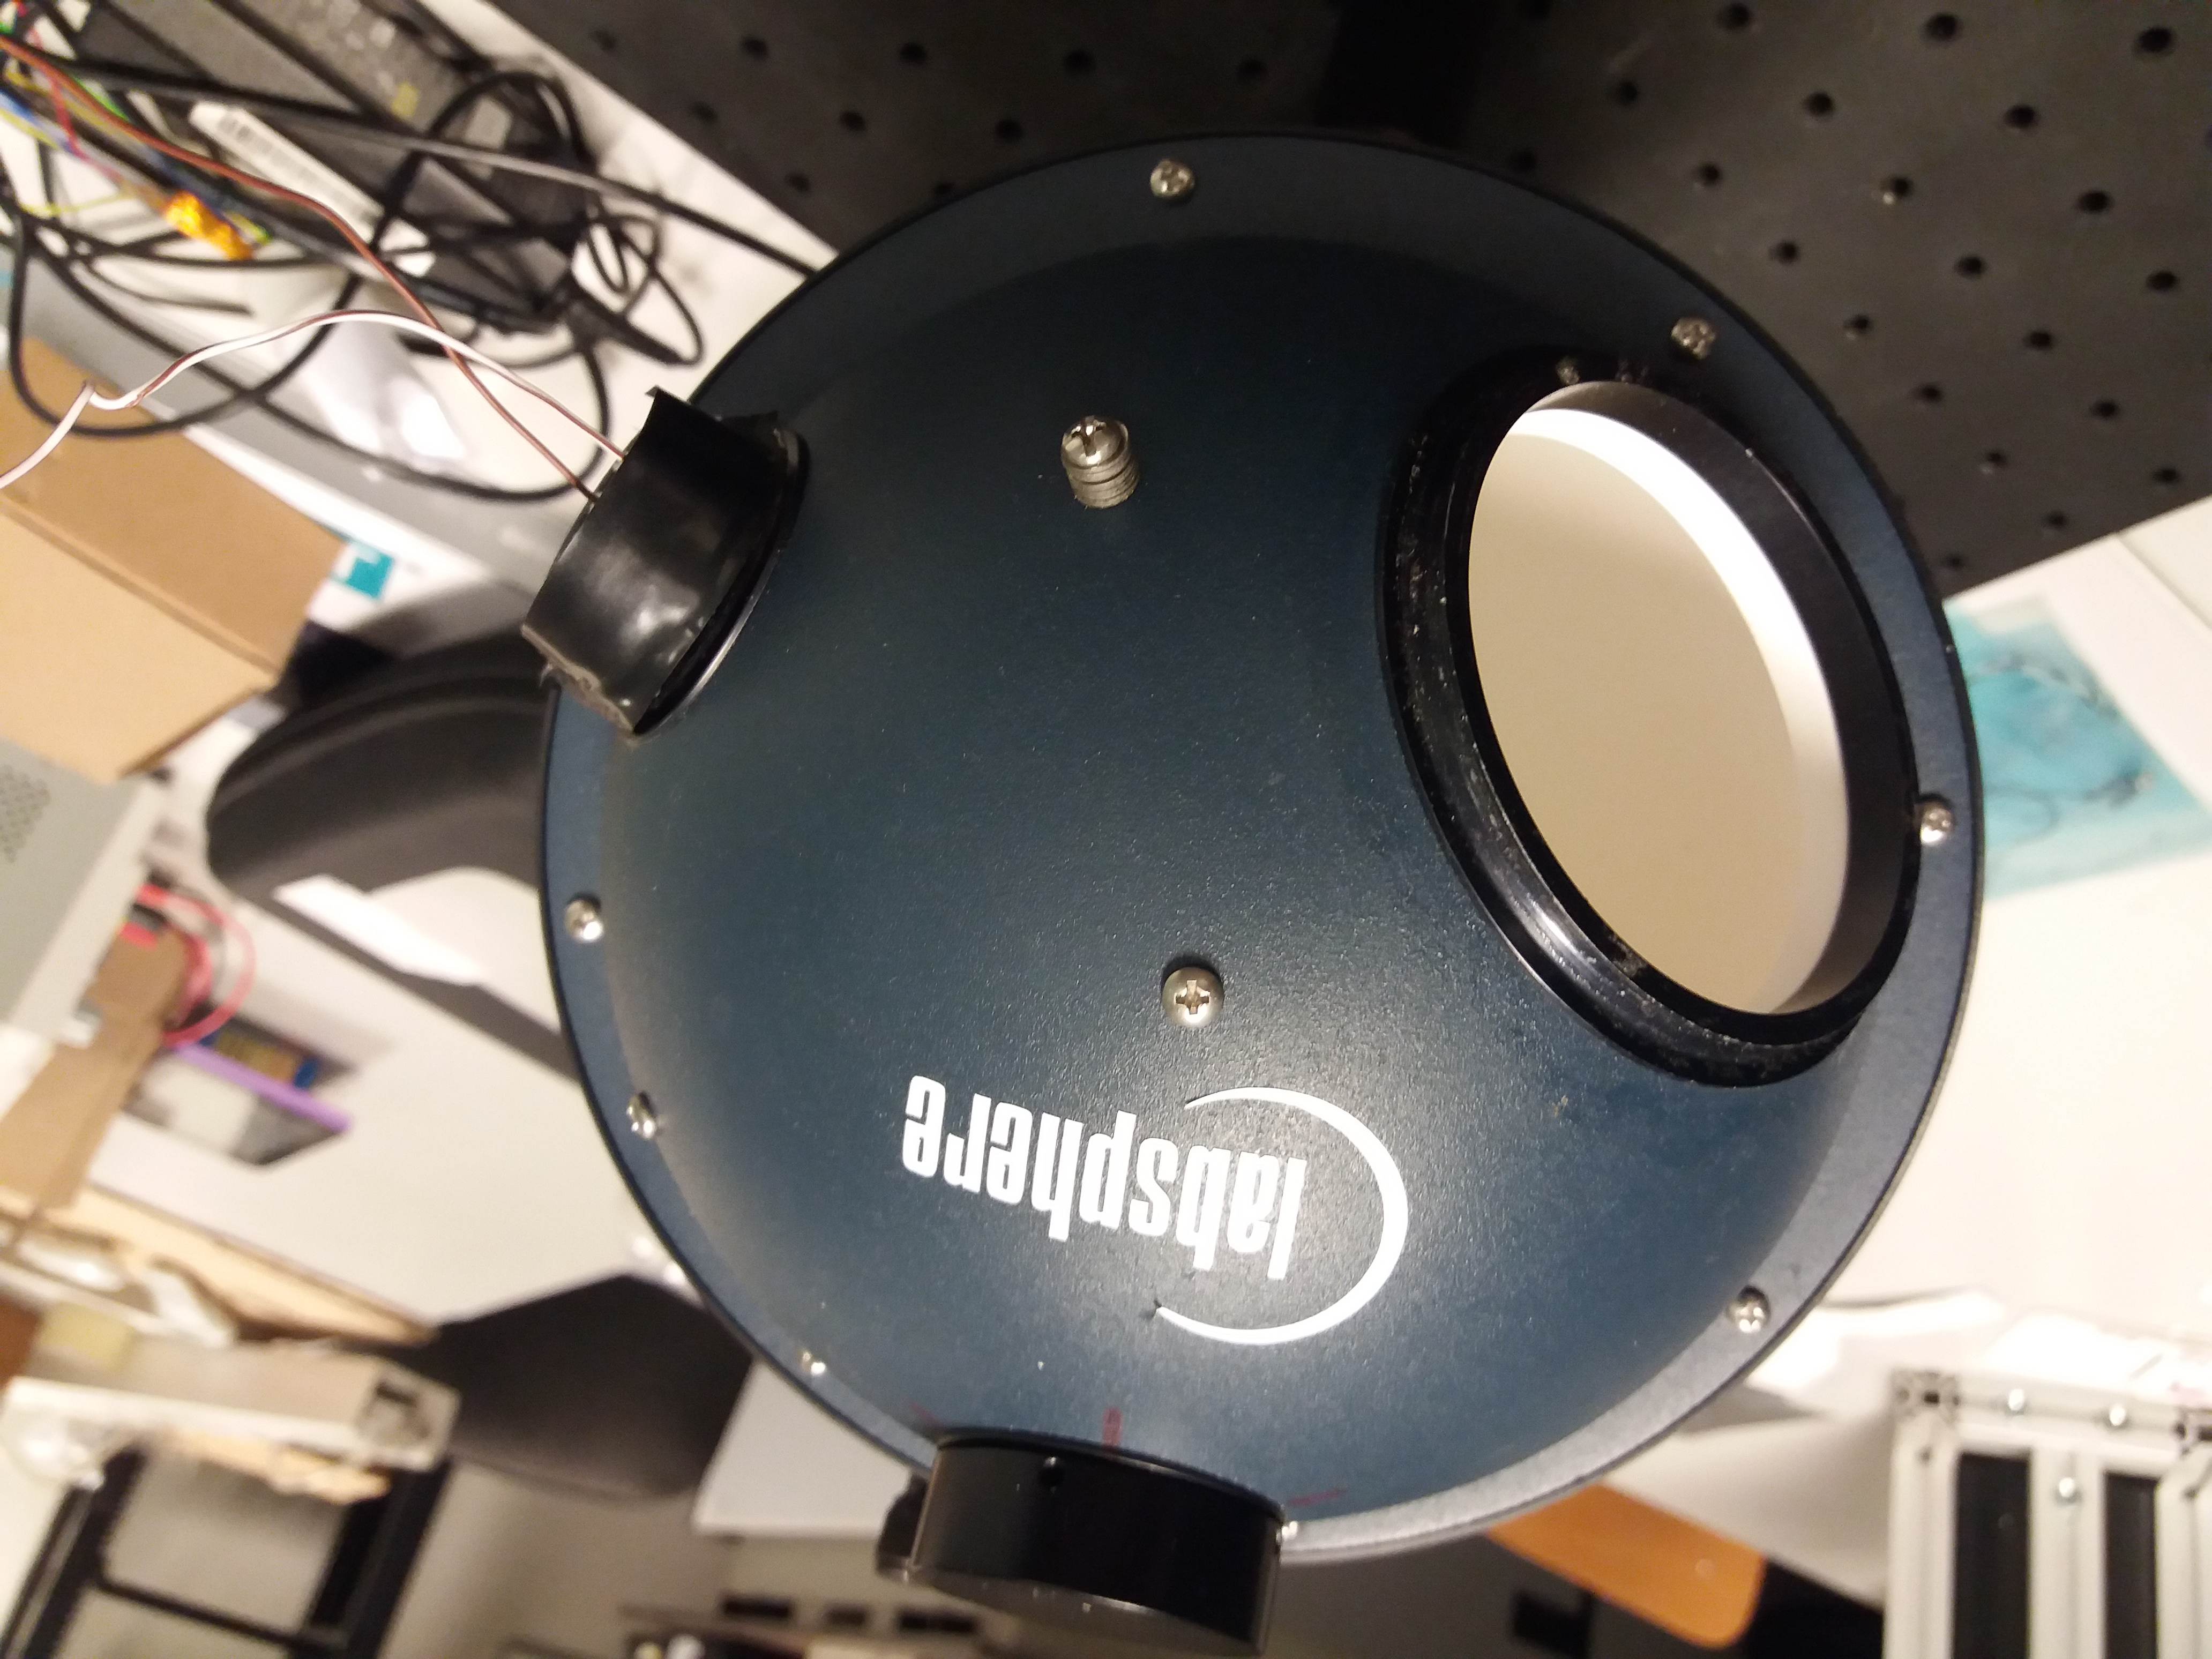
\includegraphics[scale=0.09, angle = 180]{./pictures/IntegrationSphere}
 \caption{General purpose Labsphere.}
 \label{Labsphere}
 
\end{figure}
\par
The IS inner surface consist of white optical diffusive material (BaSO$_4$ and Polytetrafluoroethylene). The IS also contains several circular apertures, which are called input/output ports. These can be used to mount detectors or optical sources or left free to let light flux enter or exit IS. 
\par
The inner surface is the part where light integration happens. The effect which takes place here is known as Lambertian scattering. After one spot of inner surface is hit by a ray, the energy should be uniformly radially distributed. In output port this produces a homogeneous light source. The homogeneity decreases with increasing number and sizes of input/output ports.
\par
Using optical source with IS typically requires baffle to prevent source's light flux or its part to exit IS without integration.
\par
Deep explanation of IS working principles and characterization of optical properties of the identical IS, which we use, can be found in \cite{VACULA2021167169}.
\par
For our purposes, in case of FAST calibration, we use IS as an UV EULS. In case of testing optical UV calibration source, we use IS mainly to block the possible incoming external light and to distribute the optical power of the UV source between mounted detectors.
% -----------------------------------------------

\section{Photomultiplier tube}
% -----------------------------------------------
Photomultiplier tube (PMT) is considered to be a high voltage optoelectronical part. It allows us to measure very low intesity optical signals. PMT is also characterized by high amplification, low noise and stability. It has many variants of usage. It can be used either as detector of optical signal (pulse or continual) for chosen wavelength or as a radiation detector. The general theory of PMTs is described in more detail in \cite{Photonis, Hamamatsu}. 
\subsection{Operating principle}
PMT consists of 6 main elements, which can be seen on scheme \ref{PMT scheme}.

\begin{figure}[H]
 \centering
 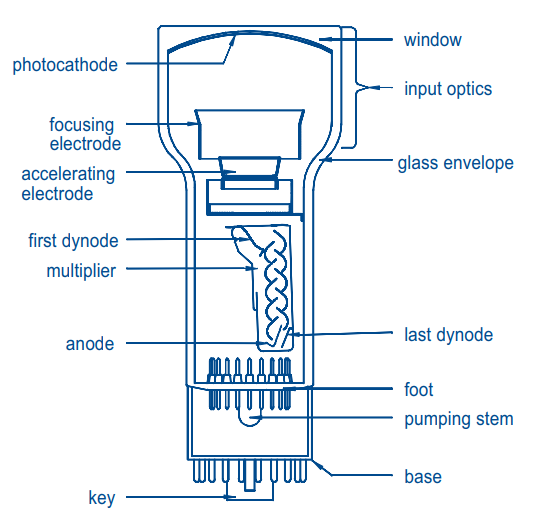
\includegraphics[scale = 0.5]{./pictures/PMTscheme}
 \caption{Photomultiplier tube scheme \cite{Photonis}.}
 \label{PMT scheme}
\end{figure}

\begin{figure}[H]
 \centering
 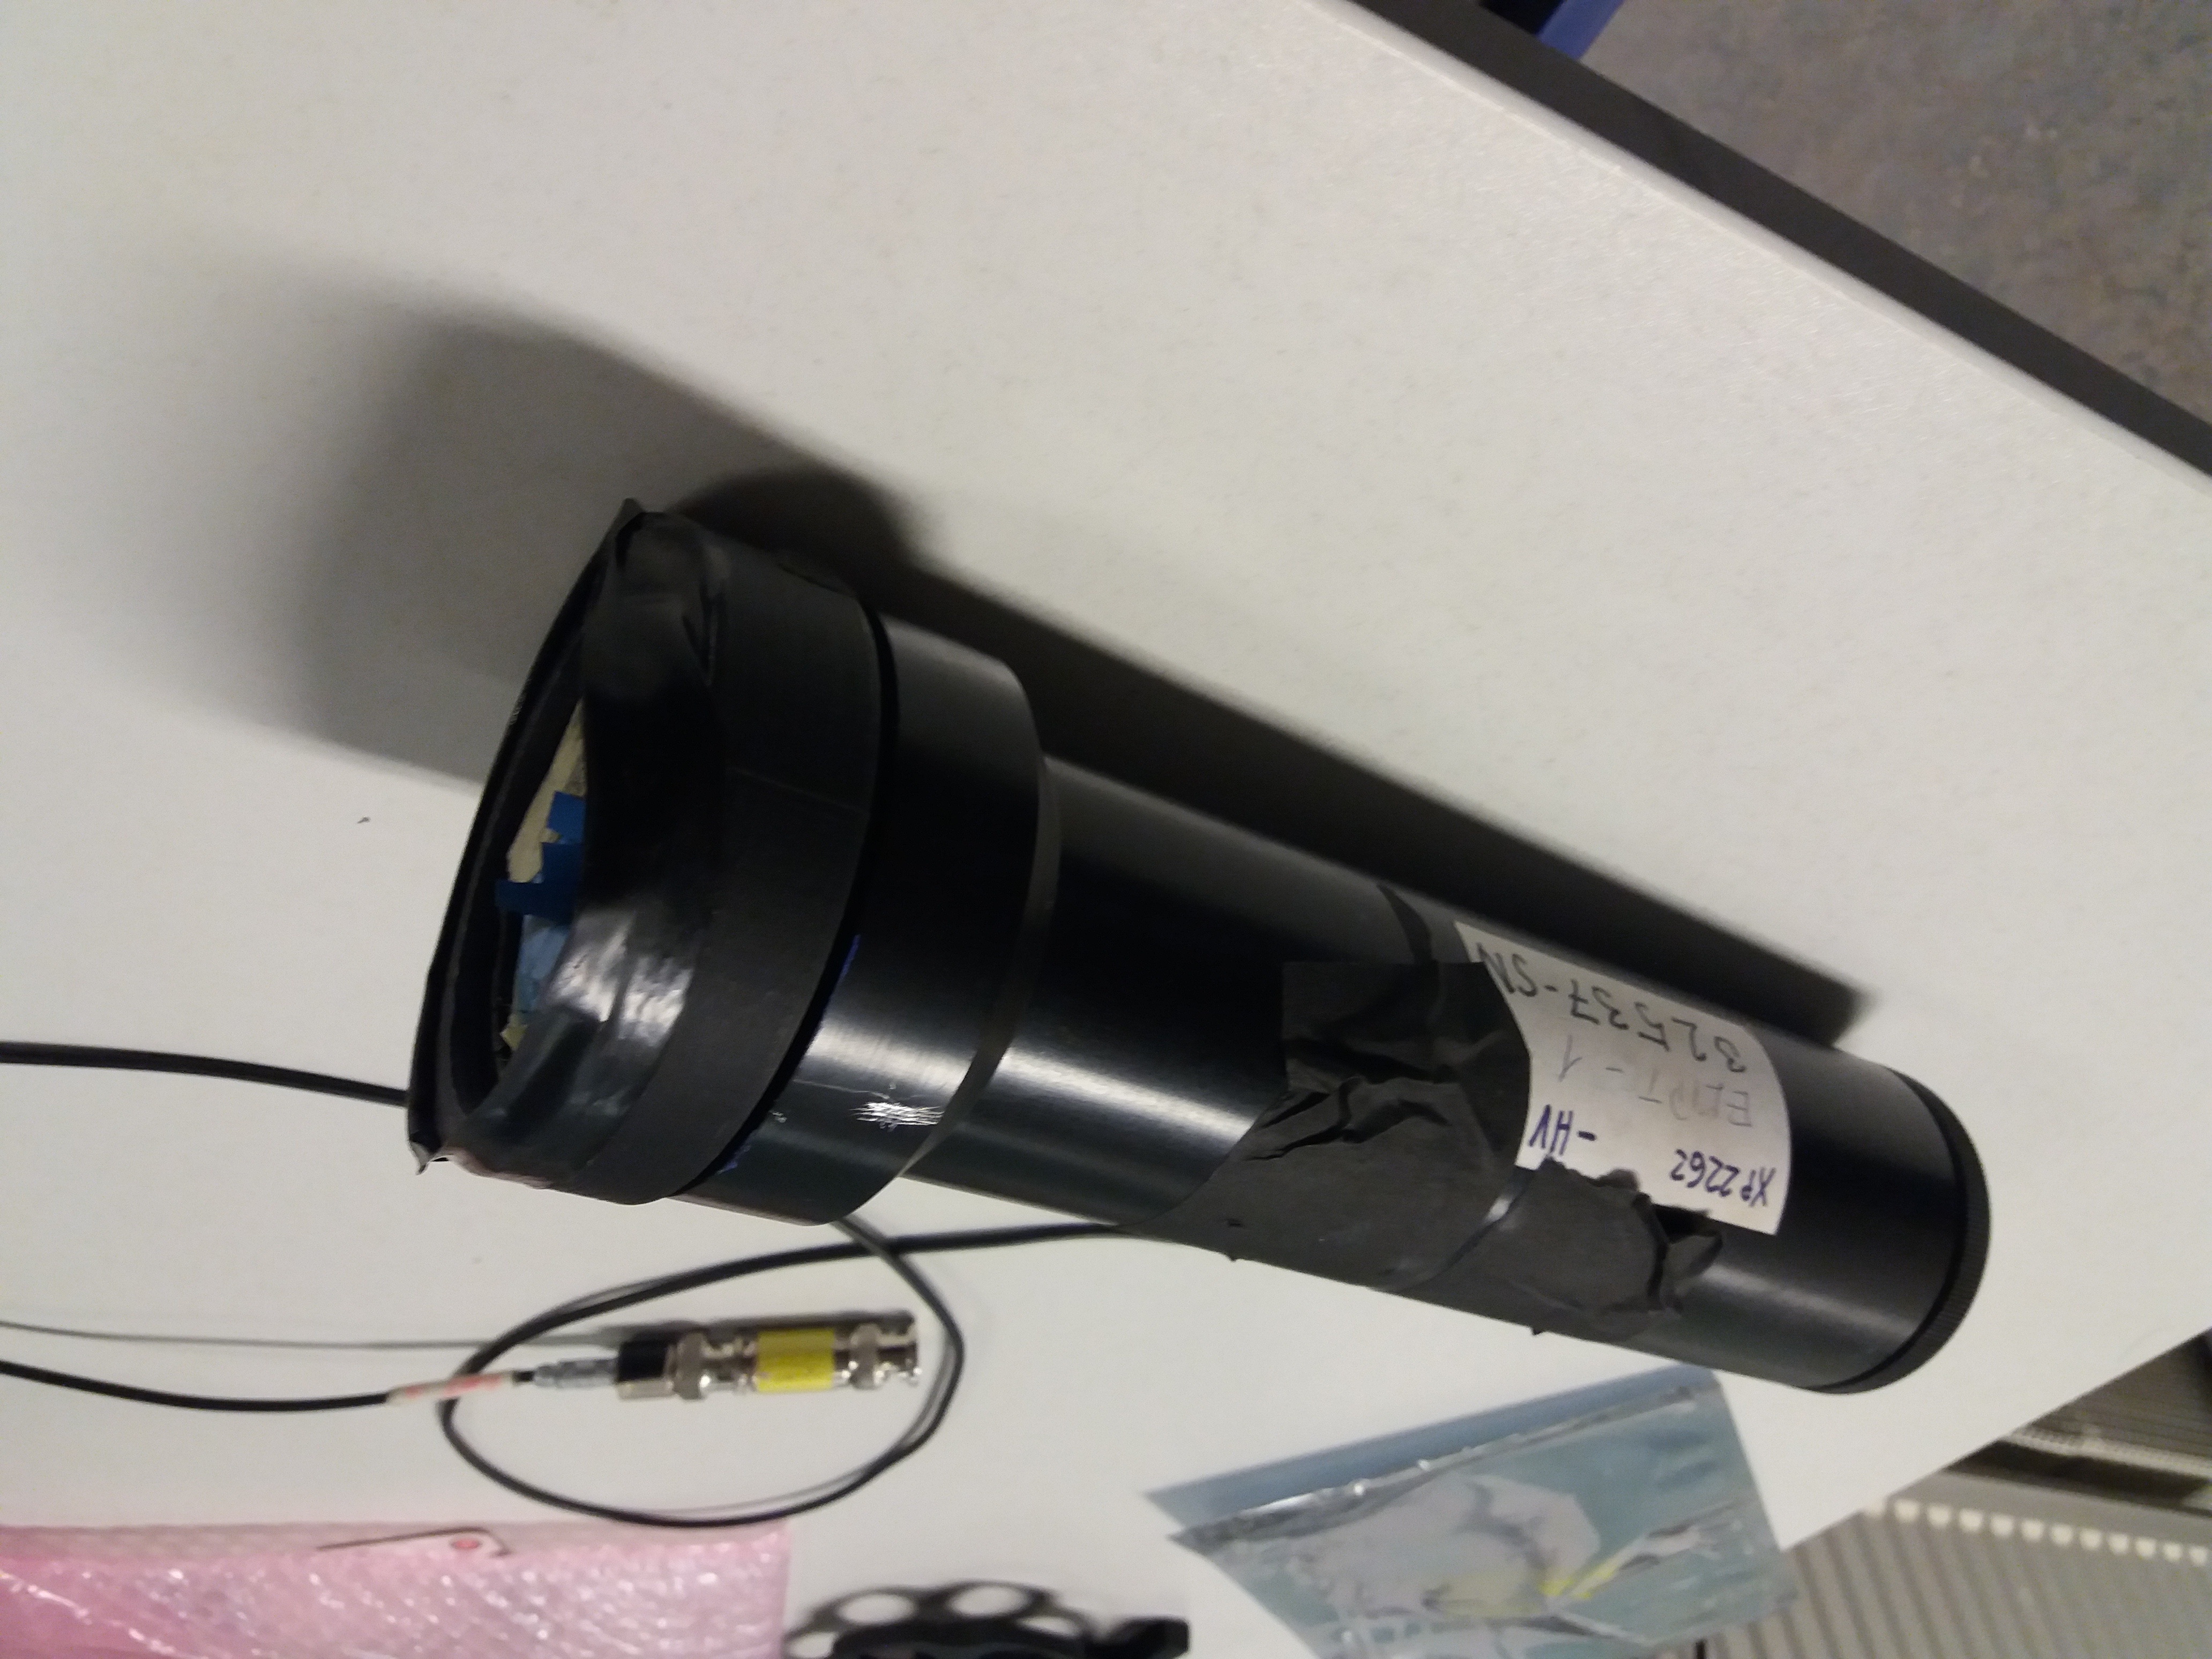
\includegraphics[scale = 0.08, angle = 180]{./pictures/XP2262}
 \caption{XP2262 PMT in a metal enclosure used for our measurements.}
 \label{XP2262 PMT}
\end{figure}

\par
The input photon with sufficient energy, which strikes the PMT's photocathode, excites photocathode's electron. This electron then follows electrostatic field to the first dynode of the electron multiplier, where it induces secondary emission of more electrons. These electrons are then attracted by the next dynode, where the emission process repeats. After few times of multiplying electron number over dynodes, the electrons are then collected by 
the anode, which is situated on the end of the electron multiplier. The anode output current is then converted to voltage signal by appropriate load resistor or by operational amplifier current-to-voltage circuit.
\par
As all other laboratory instruments, which are based on accelerating electrons, such as electron microscopes, the photomultiplier's main parts must be kept in vacuum. To maintain vacuum, the photomultiplier is surrounded by special glass envelope. To avoid mechanical damage of the glass envelope, the entire photomultiplier is sometimes situated in a plastic tube.
\par
One of the basic adjustable characteristics of PMT is its gain. The gain is defined as:

\begin{equation}
G = \frac{I_\textrm{a}}{I_\textrm{p}},
\end{equation}
where $I_\textrm{a}$ is the anode current and $I_\textrm{p}$ is the input photocurrent from the photocathode.
\par
In case of ideal, noiseless PMT, we can adjust gain by varying the supply voltage. By varying supply voltage we can adjust gain according to an equation:

\begin{equation}
\frac{G_2}{G_1} = (\frac{V_2}{V_1})^{\alpha N},
\label{gainVolt}
\end{equation}
where $G_2$ and $G_1$ are gains at supply voltages $V_2$ and $V_1$. $\alpha$ is coefficient given by dynode material and $N$ is the number of dynodes.
\par
Other effects, such as temperature, may also vary PMT's gain, and it is necessary to keep them on constant value or measure them and involve them in the final evaluation of data.
\par
For the proper functionality of the PMT, the charge and current linearity should be considered. Charge linearity is the ratio of the number of incident photons to the number of electrons collected at the anode. Current linearity expresses the proportionality between incident light flux and anode current. Ideal PMT is always linear, but the real PMT may vary from linearity due to drifts, space charges, instability of voltage divider etc. These effects can lead up to saturation of the PMT. In saturation, increasing the input light flux leaves the anode current mostly unchanged.      


\subsubsection{Window}

The photocathode is coated on glass window, whose main purpose is to admit light of certain wavelengths. Glass materials are characterized by the spectral sensitivity to wavelengths. For transparency in UV spectre, it is advised to use borosilicate or fused silica glasses.


\subsubsection{Photocathode}

The photocathode is the only light-sensitive part of PMT. It transfers the light flux into the electric current.
\par
One of its main parameters is quantum efficiency. It is referred to as ratio of emitted photoelectrons to the number of incident photons expressed as a percentage. It is generally less than 35 \%. For measurement, the more practical parameter is cathode radiant sensitivity. It is the ratio of photocathode current to an incident light power, which is expressed in mA/W.
\par
Photocathode material must be sensitive to certain wavelengths, which we want to detect with the PMT, and must have sufficient quantum efficiency. Preferred materials are usually alkali antinodes.
\subsubsection{Electron multiplier}
The electron multiplier consists of dynodes and one anode.
Dynodes are electrodes, which produce more electrons through secondary emission. To maintain electrostatic field between dynodes, each of dynodes is held on different potential. This is achieved by using the voltage divider. Every resistor in the divider sets the potential of one diode according to its resistivity.
\par
All of the photoelectrons emitted by photocathode should be ideally collected by the first dynode. However, many of them could be diverted from their path to dynode due to various effects. The parameter, which characterizes this, is the collection efficiency. The collection efficiency is probability that a photoelectron will strike area of the first dynode. 
\par
There are few types of dynodes arrangements. On the fig. \ref{PMT scheme} is the classic linear-focusing multiplier. 


\subsubsection{Voltage divider and voltage adjustment}
Voltage divider could be a simple resistor serial network, which divide high input voltage between the dynodes. 
\par
It is necessary to consider, that the multiplier current density increases in direction to the anode, so it tends to lessen the voltage between last dynode and anode. This phenomena can shake the potential levels across the entire multiplier. One way to reduce the impact on PMT's behaviour is to choose the proper resistor values of the divider. 
\par
The resistor values could same for all the dynodes, but for some applications it is better to have progressive voltage distribution, which increases from cathode to anode, or intermediate distribution with highest values on the beginning of the multiplier.

\par
In some applications, where high anode current peaks are expected, the divider can be filled with reservoir capacitors, which prevent the temporally charge exhaustion of the dynodes. In pulse mode, the unwanted oscillations on dynodes may occur, in that case, it is desirable to connect additional damping resistor to the divider.
\par
Voltage supply should be stable during the PMT's operation. As was mentioned before, the PMT's gain is voltage dependent. To adjust sufficient gain, high voltage (hundreds of volts) needs to be applied between photocathode and anode. The high voltage needs to be ramped on required level gradually to avoid negative consequences of transition and dark current effects, which can decrease the operating life of PMT. The same is valid for shutting down the PMT.
\par
The high voltage could be applied to the PMT in negative or positive polarity. In case of positive polarity, the cathode is held at ground and anode on +HV. In case of negative polarity, the cathode is held at -HV and anode at ground. 

\subsection{Dark current}
Dark current is the anode current produced by a photomultiplier in total darkness. It is considered to be a part of unwanted noise, causes errors in measurements and limits the detectivity of PMT. Dark current has origin in ohmical leakage, thermionic and field emission or in radioactivity. Ohmical leakage is major part of dark current at low gain. With the increasing gain the thermionic emission prevails. At high gains the field emission becomes the major part.
%\subsubsection{Ohmical leakage}
%Insufficent insulation of electrodes, dynodes and all other parts which are under high voltage may lead to surface current over glass and tube. Dirt and humidity are in most cases the reason of Ohmical leakage.

%\subsubsection{Thermionic emission}
%Temperature causes emission of photocathode's electrons, which are at medium gains the major part of dark current.  Due to this effect, some PMTs may need to be cooled during operation.
%\subsubsection{Field emission}
%At high gains the electrostatic field is so strong that it can rip the electrons out of the electrodes and accelerate them onto other surfaces, where they cause secondary emission. Field emission rapidly increases with supply voltage. In some literature it is also refered as cold emission.
%\subsubsection{Radioactivity}
%The radioactivity of PMT's components depends only on the material composition. In some aplications, such as astroparticle detection, it is neccessary to decrease radiation as possible. In astroparticle detection the radioactivity could be a source of false events. Only way to prevent this is to use materials with a very low concentration of radioactive isotopes.

\subsection{Timing and response}
Differences of photoelectrons' trajectories from the cathode to the first dynode lead into time distortion of signal. For example if we were able to produce delta-function pulse, the PMT would detect pulse with some response width time $t_\textrm{w}$.
With respect to differences in electron trajectories and arrival times, the PMTs are divided into 3 types:
\begin{enumerate}
\item \textbf{Very-fast tubes} - photoelectrons arrive simultaneously, low collection efficiency.
\item \textbf{Fast tubes} - compromise between timing performance and collection efficiency
\item \textbf{General-purpose tubes} - simple optoelectronics, good collection efficiency, low timing performance
\end{enumerate}
%\par 
%Another time delay to be considered 

\subsection{Operating life and degradation}
The operating life of PMT is defined as the time required for anode sensitivity to be halved. If we neglect the outside effects, the operating life mainly depends on anode current. 
Degradation processes start to show themselves at currents higher than 10 $\mu$A. Ageing is accompanied by increasing or decreasing gain at stable voltage. Operating life of PMT is measured in thousands of operating hours.
\par
By exposing PMT to bad conditions, such as humidity, mechanical stress, high temperatures or the high-intensity light, the PMT's operating life could be shorten much faster.
%------------------------------------------------
%------------------------------------------------

\section{Hardware for experiment control}
% -----------------------------------------------

\subsection{Raspberry Pi}
Raspberry Pi (RPi) is a single board computer which we use mainly for the experiment control. The linux-based Raspbian or DietPi operating system allows us to easily run various scripts and programs written in multiple languages. By having wifi and an ethernet port, the RPi can be easily accessed over internet. It can be used to control instruments and data acquisition over its USBs,1-Wire and I2C etc. However, it doesn't have any analog inputs/outputs such as ADCs and DACs.
\subsection{STM32 based microcontrolers}
For other types of tasks, which do not require data storage and remote control, but require for example an analog sampling, setting up the voltage levels or generating well defined PWM pulses, we use STM32 based microcontrollers. 
\par
For this thesis purposes we use the STM32 nucleo F411RE and the STM32 nucleo F446RE with better analog inputs/outputs.
% -----------------------------------------------
% %%%%%%%%%%%%%%%%%%%%%%%% End of file %%%%%%%%%%%%%%%%%%%%%%%%

% -----------------------------------------------
% -----------------------------------------------
% Vlastní text práce (kapitoly práce)
% -----------------------------------------------

% -----------------------------------------------
\chapter{Calibration UV optical source}
% -----------------------------------------------
 \label{chap4}
As was mentioned before, the calibration UV optical source is an essential instrument to perform calibrations. Its main purpose is to deliver stable intensity which does not vary over time or due to the changes in outer conditions.
\par
In case of FAST the process of calibration requires low-intensity UV light to be delivered in microsecond square pulses. This is because FAST is a low-intensity detector and its PMTs may be easily saturated.

% -----------------------------------------------
\section{UV source}
% -----------------------------------------------
For the calibration purposes a prototype of pulse UV source was developed. It was based on the current-driven LEDs inspired by the Karlsruhe Institute of Technology (KIT) concept. The active parts - LED drive circuit and 3 LEDs are situated in temperature stabilized head. 
\par
The source is driven by STM32 board, which allows us to set parameters - LED current by setting the voltage on the DAC channel, PWM duty and frequency, which is used to excite LED current through op amps.
 


 \begin{figure}[H]
 \centering
 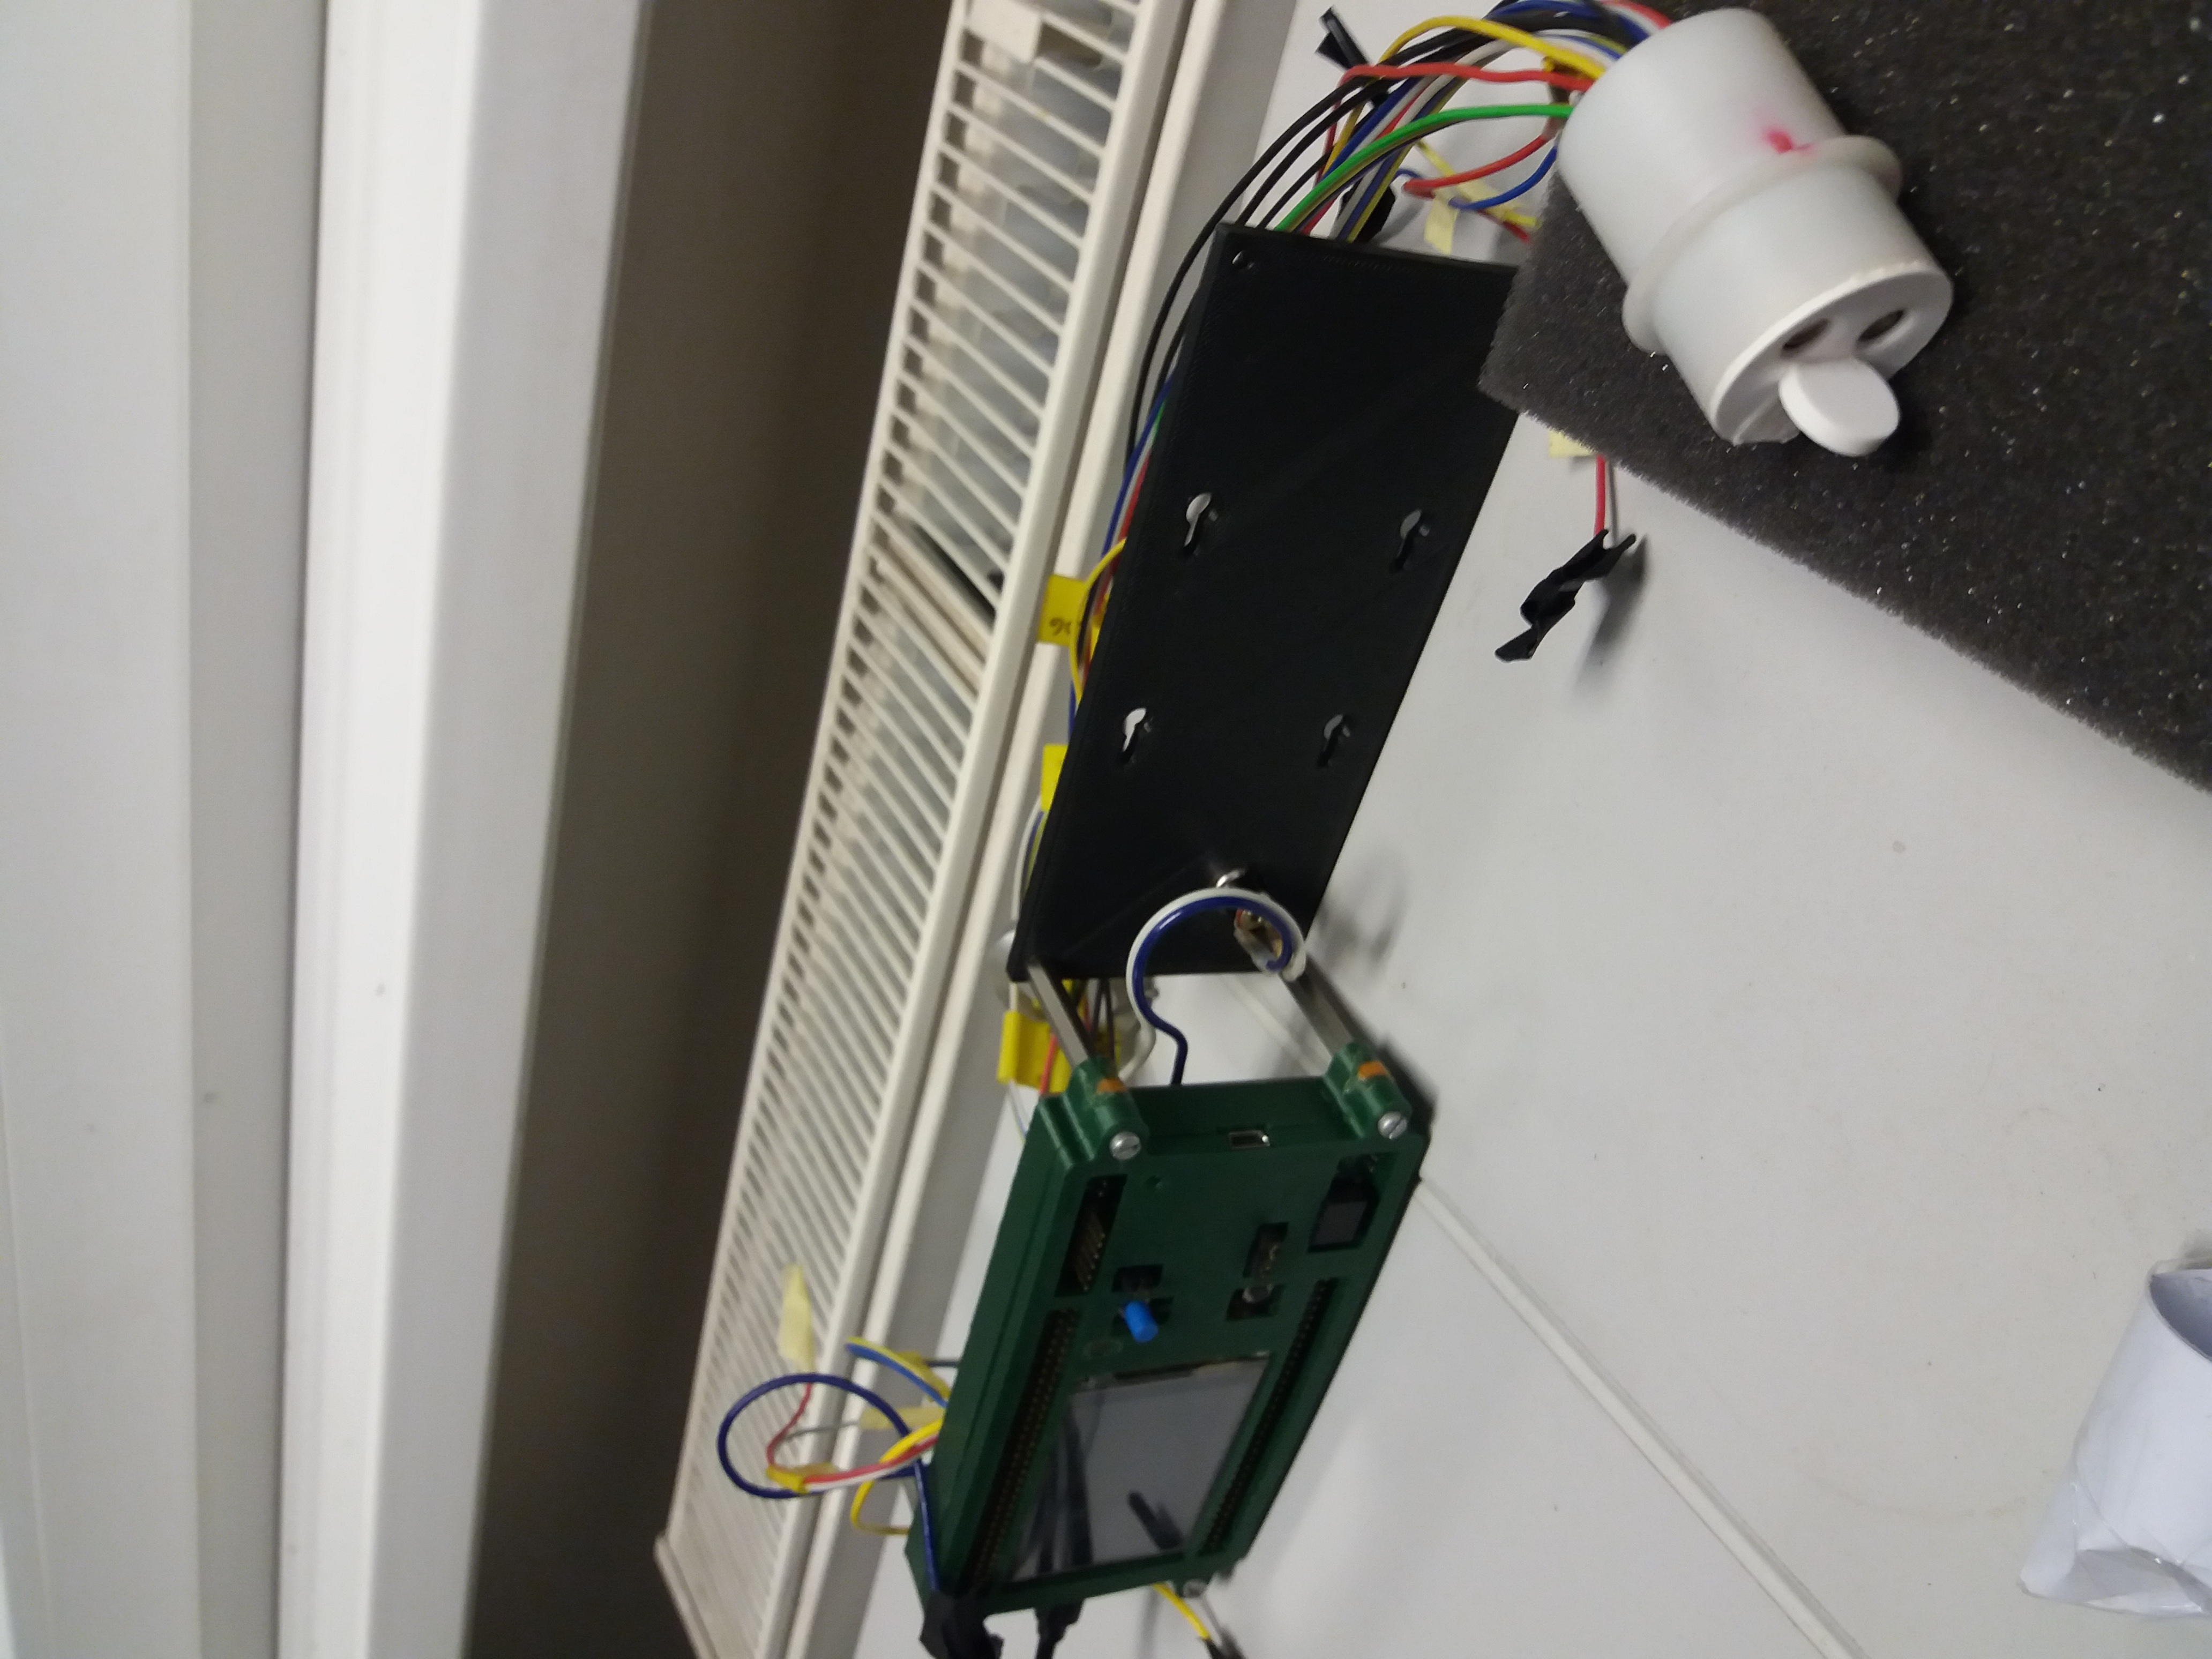
\includegraphics[scale=0.09, angle = 270, origin = c]{./pictures/KarlsRuhe}
 \caption{UV source constructed by Vladimír Urbášek from Jointlab.}
 \label{UVsource}
\end{figure}

 \begin{figure}[H]
 \centering
 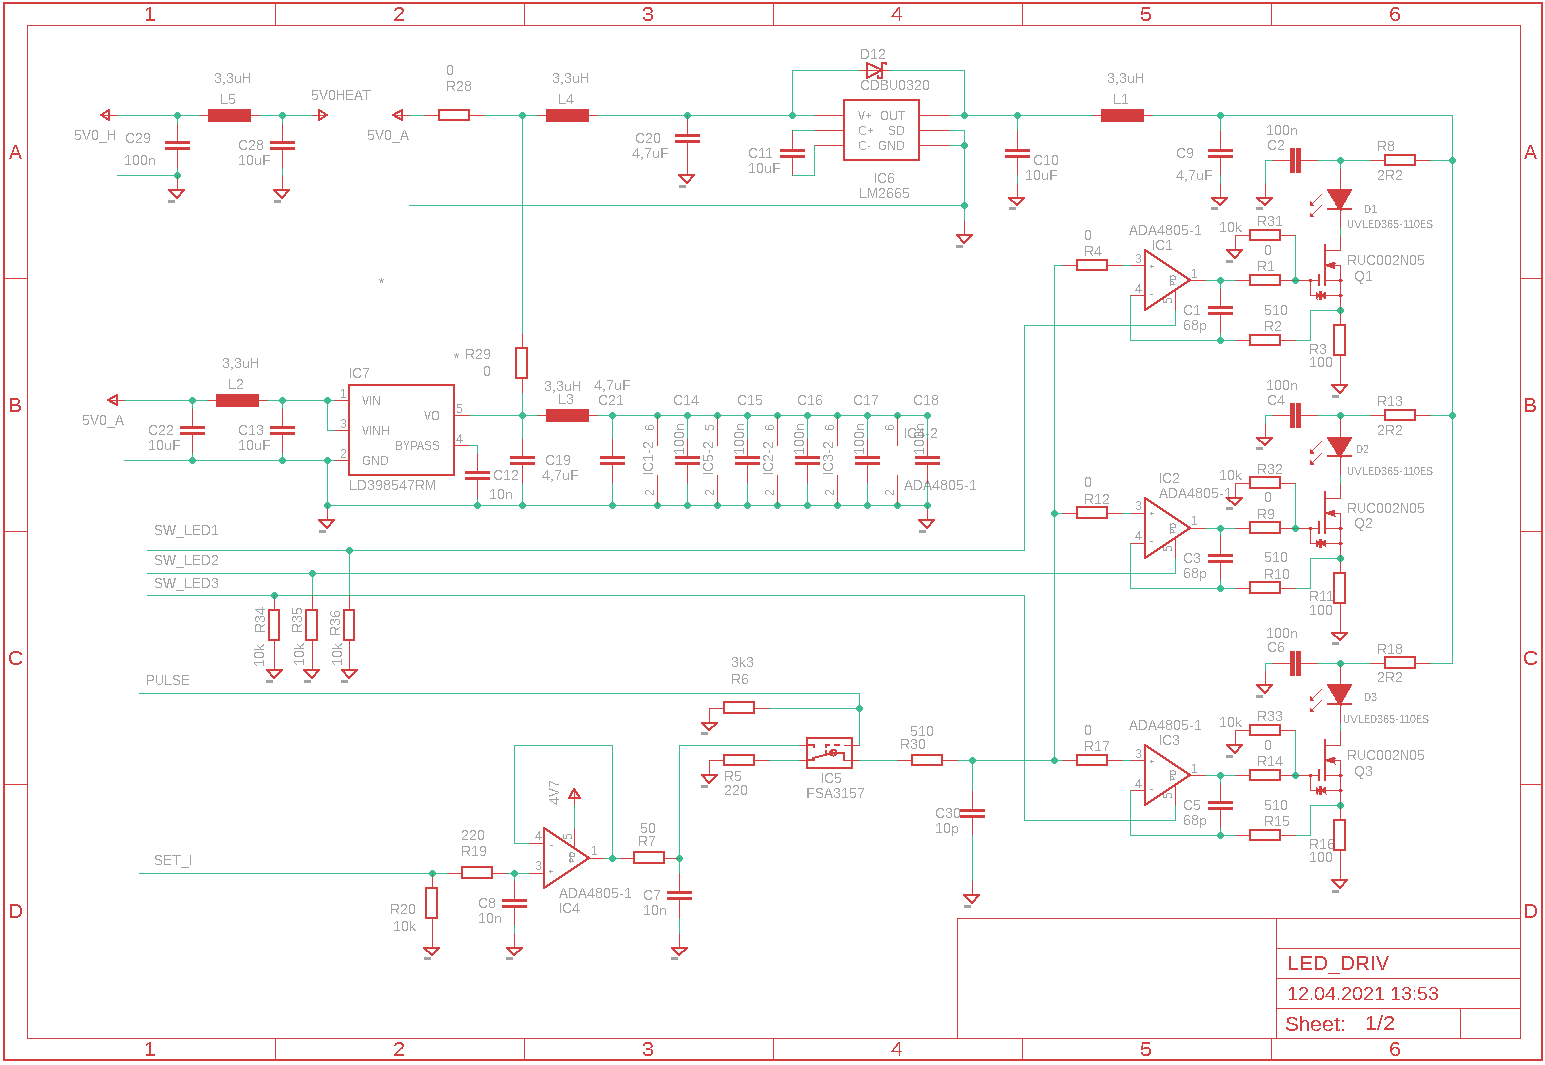
\includegraphics[scale=0.5, angle = 0, origin = c]{./pictures/OrigScheme.png}
 \caption{UV source schematic. On the right side we can see the pulse current drivers for three LEDs with the feedback Op amps as the main component.}
 \label{UVsource}
\end{figure}


Our main task was to test this UV source's long-time stability and develop possible fixes and upgrades.

% -----------------------------------------------

\section{Testing and measurement of UV source}
% -----------------------------------------------
For calibration UV source, the long-time stability of optical power and pulse geometry is very important. Because there was no specialized apparatus for this measurement, we had to make our own. For these measurements, we use UV source with LED current $I_{\textrm{d}}$ = 2.5 mA, 50$\%$ duty cycle and frequency $f = 50$ kHz. 
\subsection{Measuring apparatus}
For measuring the optical power we use PM16 power meter (PM) and for determining the pulse geometry we use XP2262 PMT with signal output connected to 2-channel PicoScope 2205A MSO usb oscilloscope. XP2262 PMT is held on $U \approx -680$ V by HV voltage source. The PMT's gain may drift over time, but we use PMT mainly for geometry analysis and measurement of absolute optical power is left to PM16.
\par
We also use DS18B20 thermometer for PMT temperature monitoring and keysight 34461a multimeter for readout of voltages.

\par
The PMT, power meter and the optical head of UV source are mounted in the IS's ports. The IS stops the unwanted external light and distributes the optical power to PMT and power meter. 
\par
The entire apparatus is controlled by Raspberry Pi (RPi). The RPi takes care of data acquisition and can be used to set the parameters of the UV source. It can be easily accessed over internet for data download or for user to control the experiment.
\par
Osciloscope's readout was programmed in C language according to its programmer's manual \cite{PicoScope}. It is capable of 2ns sampling which is enough to capture rising edges of the pulses. The RPi sets basic parameters (DC coupling, range etc.) and then activates oscilloscope's trigger (rising edge). After sampling, RPi receives all samples from oscilloscope's memory.
\par
The multimeter is controlled by VISA commands using python USBTMC library. For thermometer we use RPi's 1-Wire.
\par
Main component (IS,PW, PMT with HV source, UV source) are situated in protection box to prevent unwanted manipulations and touching the HV parts.The apparatus can be seen on Fig. \ref{aparature1} and \ref{aparature2}.

\begin{figure}[H]
 \centering
 \includegraphics[width=150mm]{./pictures/aprature1b}
 \caption{Measuring apparatus.}
 \label{aparature1}
\end{figure}

\begin{figure}[H]
 \centering
 \includegraphics[scale = 0.09]{./pictures/aparature2b}
 \caption{PMT mounting and HV source.}
 \label{aparature2}
\end{figure}


\subsection{Data acquisition and analysis}
All the data are taken in specified interval (15 or 30 minutes). Two files are produced - osciloscope waveform file and a file with 30 samples of power meter, multimeter and a thermometer readings. From these 30 samples we calculate average and error. Most of data analysis we perform is done by C/C++ Root framework \cite{ROOT}.
\par
The data from oscilloscope contains the square pulses with noise (Fig. \ref{pulse}). From them we need to extract the information of pulses height, slope and time of the rising edge.

 \begin{figure}[H]
 \centering
 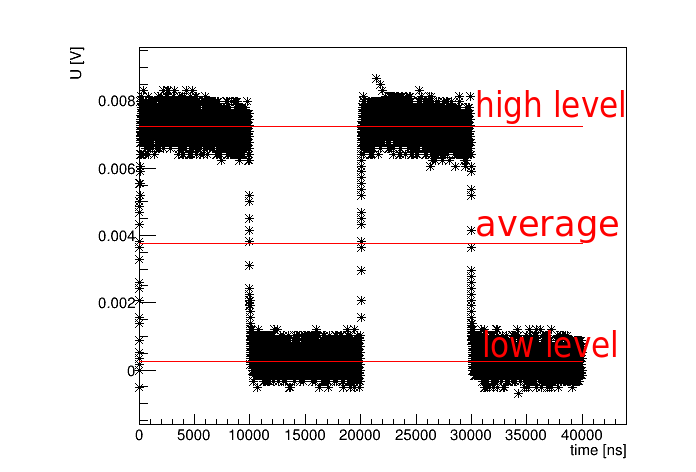
\includegraphics[scale=0.65]{./pictures/PMTPulse}
 \caption{Determining the basic pulse properties - average, low and high levels of signal.}
 \label{pulse}
\end{figure}

To determine the pulse height, we need to calculate the average value from all the samples at first. Then, we split the samples into two subgroups according to fact, whether they are higher or lower than the average. These subgroups are converted to histograms with fixed binning (around 5000 bins). These histograms are then fitted by gaussian. The means of these two fits determine two levels of the pulse - high ($U_\textrm{h}$) and low ($U_\textrm{l}$). The Fig. \ref{pulse} shows the real pulse with levels determined by this method. The height of pulse is then simply calculated by subtracting two levels: $U_\textrm{H} = U_\textrm{h} - U_\textrm{l}$.

\par
The properties of the rising edge can be specified by two parameters, which we are able to extract from our data - time and the slope of the rising edge. We are able to calculate both of them if we identify the samples of the rising edge. These samples' values should be between 20 $\%$ and 80 $\%$ of the $U_{H}$. First, we need to detect the rising edge in waveform data sequence. However, the signal is very noisy and this can not be simply done by detecting the exceeding of the 10 $\%$ of the $U_{H}$ .To achieve that, we cycle through the waveform until we meet two conditions - the value is higher than average (and lesser than $80 \%$) and the derivative is positive. Due to the noise, the derivative could not be calculated from two or three points, thus we use Savitzky–Golay polynomial's derivative at chosen point: $y' = \frac{1}{12h}(y_{i-2} -8y_{i-1} + 8y_{i+1} - y_{i+2}) $. However we care only of positive/negative sign, so $\frac{1}{12h}$, where $h$ is the small step, is no use for us. When these two conditions are met at some point, the program cycles back from the point through the waveform until reaches $20\%$ level, and then beginning at the same point, which met the conditions, cycles up to reaching $80\%$ level. All the samples traversed by this way are considered as samples of the rising edge. The rising time is calculated simply by multiplying the number of these samples by the sample time (2 ns). The slope is calculated from linear fit of these samples (Fig. \ref{linfit}).  


 \begin{figure}[H]
 \centering
 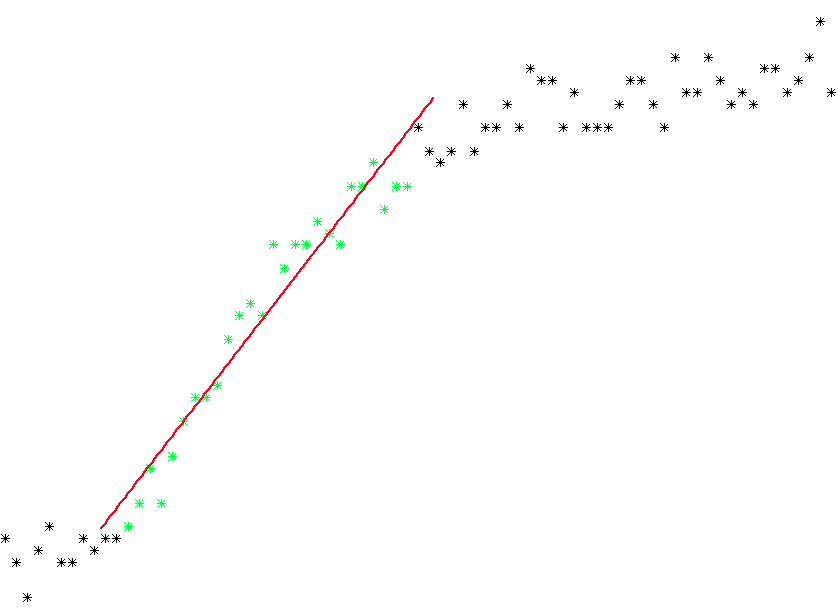
\includegraphics[scale=0.35]{./pictures/linFit}
 \caption{Linear fit of rising edge points (marked as green).}
 \label{linfit}
\end{figure}


\subsection{Results}
First data taking sequence ran about two weeks. Taken data were analysed by methods described in previous chapter and results are presented in the following graphs. The first two graphs describe 
optical power with respect to time (first from PM and second is the PMT pulse height).
\begin{figure}[H]
 \centering
 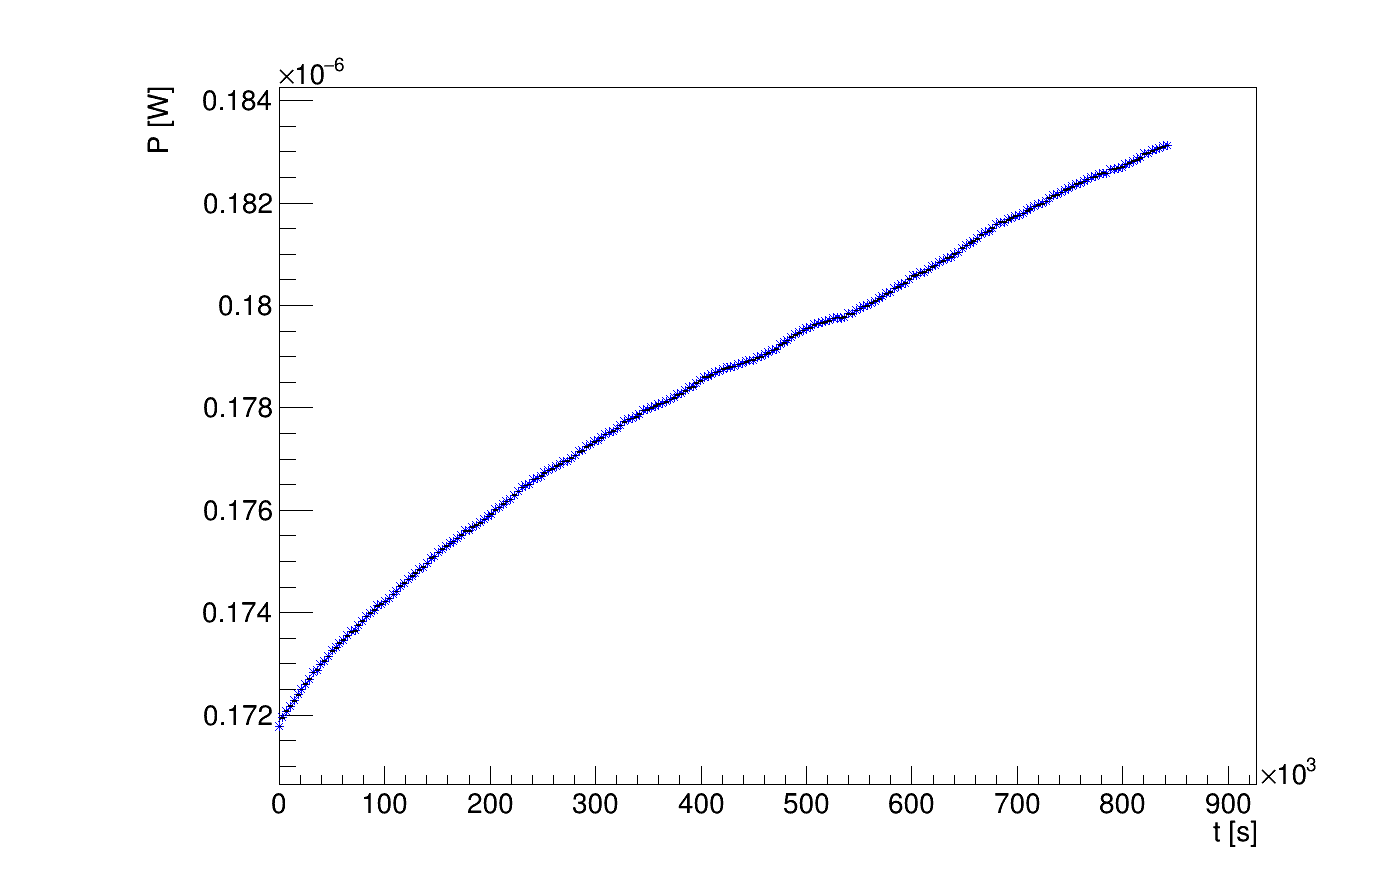
\includegraphics[scale=0.3]{./pictures/powers}
 \caption{Time evolution of optical power.}
 \label{pow1}
\end{figure}



\begin{figure}[H]
 \centering
 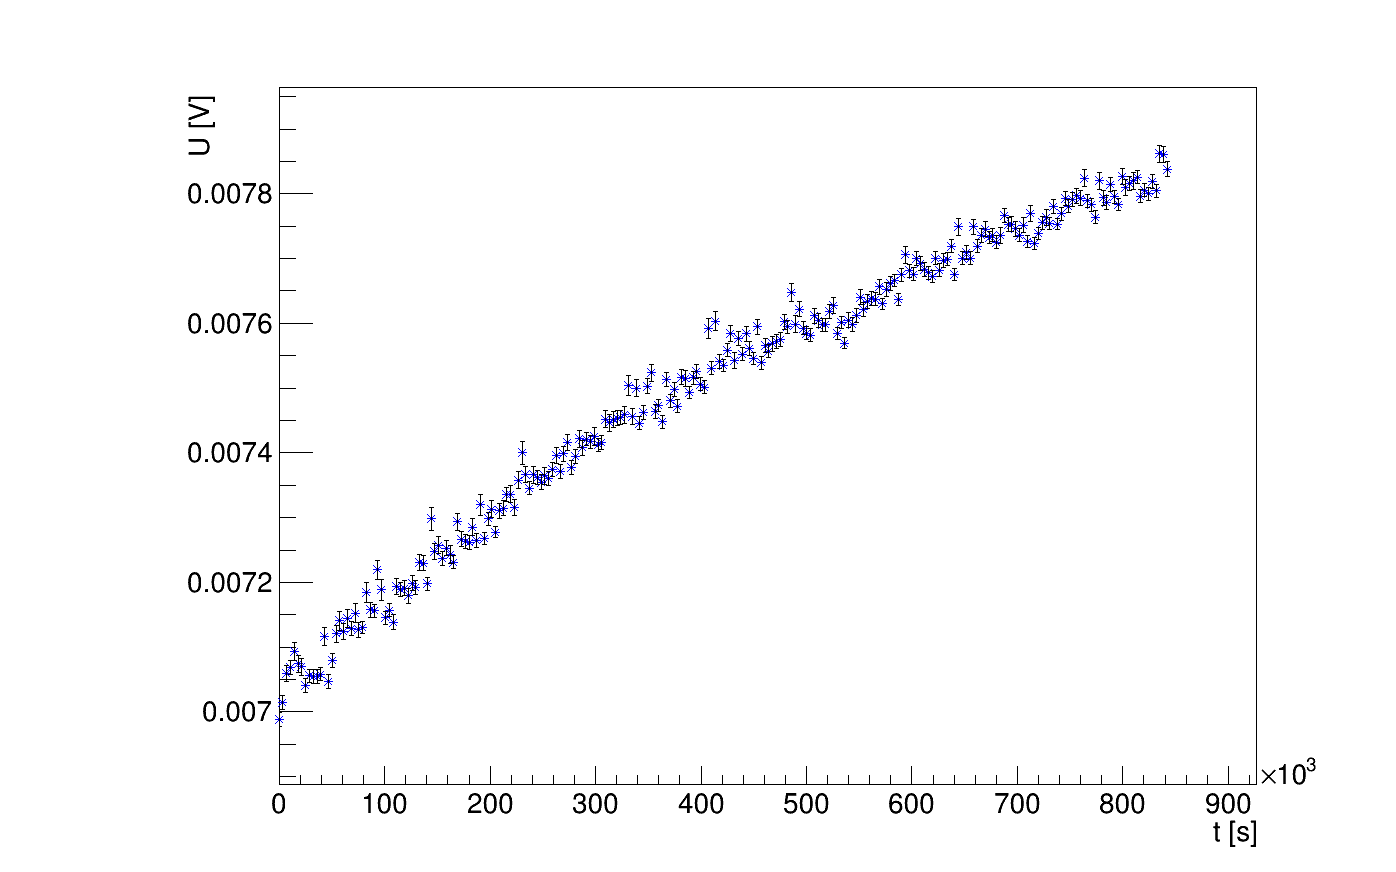
\includegraphics[scale=0.3]{./pictures/Height}
 \caption{Time evolution of the pulse's height.}
 \label{height1}
\end{figure}

In the next two graphs we present calculated heights and slopes.

\begin{figure}[H]
 \centering
 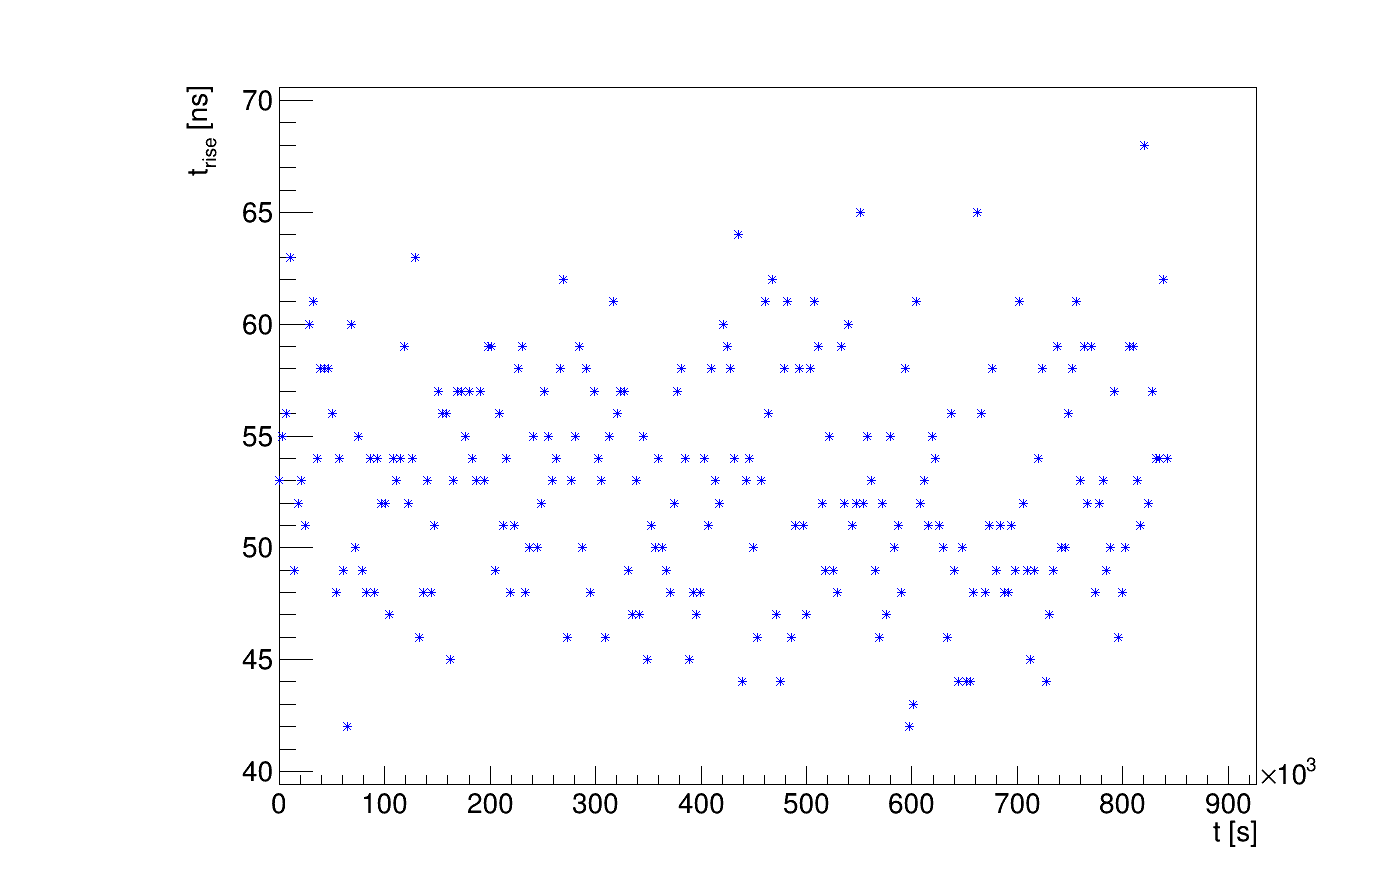
\includegraphics[scale=0.3]{./pictures/rise}
 \caption{Time evolution of the pulse's edge rise time.}
 \label{rise1}
\end{figure}

\begin{figure}[H]
 \centering
 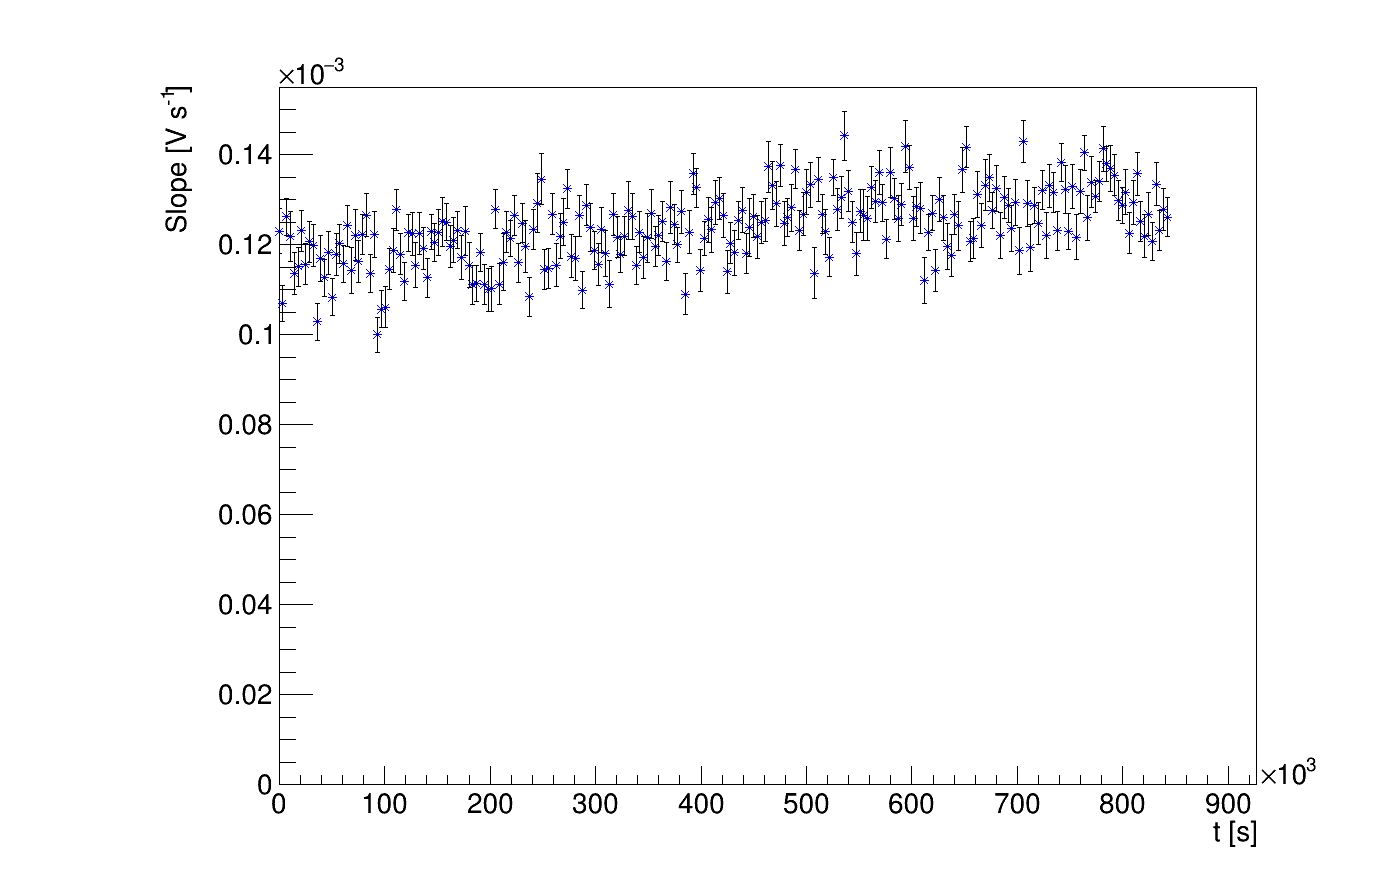
\includegraphics[scale=0.3]{./pictures/Slope}
 \caption{Time evolution of the pulse's edge slope.}
 \label{slope1}
\end{figure}

We also measured PMT's temperature for potential corrections.
 
\begin{figure}[H]
 \centering
 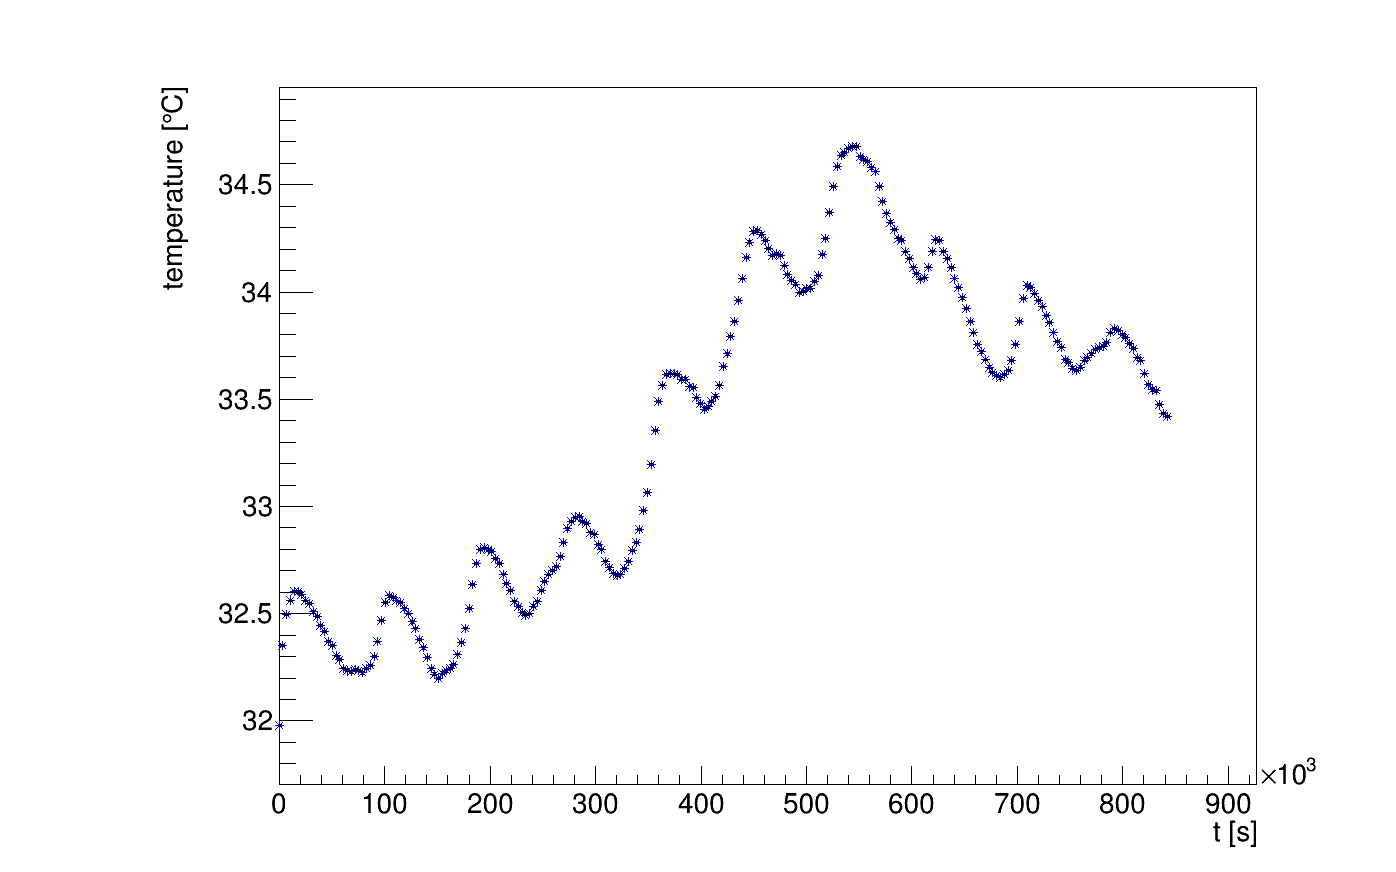
\includegraphics[scale=0.3]{./pictures/temperatures}
 \caption{Time evolution of the PMT's temperature.}
 \label{temp1}
\end{figure}

From analysed data we may observe that the power is rising over time. This fact is confirmed by two sensors - both PM and PMT. In case of PMT there may be the drift in gain over time. Gain drift may be caused by changes in voltage (equation \ref{gainVolt}) or in temperature. In case of temperature, the trend is not only rising as $U_{H}$'s trend does, so the $2_{\circ}$ change in temperature may play little role in $U_{H}$ increase, but it is not probably the main cause of this effect.
The graphs \ref{rise1} and \ref{slope1} shows that pulse is not deforming over time.
\par
The optical power instability may be caused by failures in LED driving circuit (changes in current flowing by diode) or by ageing processes in the UV diodes. The PM shows that the power increase is around $7 \%$ in 10 days, which is unacceptable for any calibration source. 
\par
To confirm this measured fact and check for possible causes of the optical power instability we repeated this measurement by few times with similar results. But during these measurements we used multimeter to monitor PMT's voltage. For measuring the current flowing by the diode in the internal current source circuit, we used the second channel of the osciloscope.

\begin{figure}[H]
 \centering
 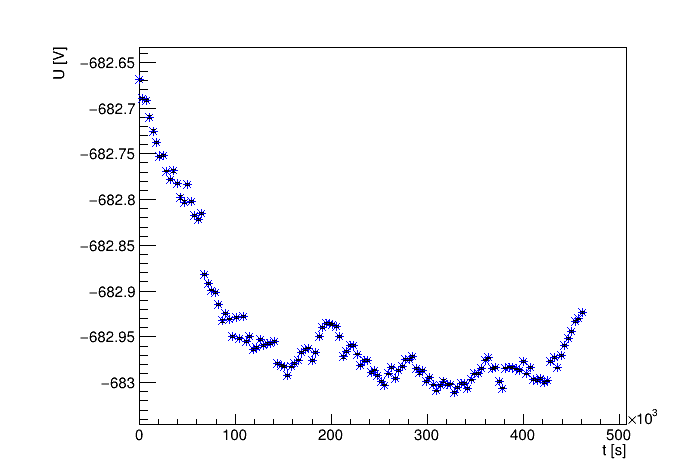
\includegraphics[scale=0.5]{./pictures/voltage}
 \caption{Time evolution of the PMT's voltage.}
 \label{PMTVolt}
\end{figure}

\begin{figure}[H]
 \centering
 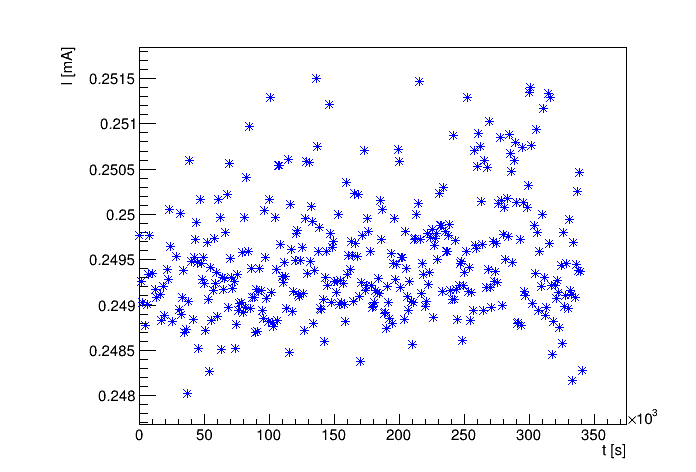
\includegraphics[scale=0.5]{./pictures/Current}
 \caption{Time evolution of the UV LED's current.}
 \label{LEDCurrent}
\end{figure}

Other measurements of optical power have ended in similar way. But by using the multimeter we can see that PMT's voltage is stable (Fig. \ref{PMTVolt}). It is varying only about 0.4 V at the beginning.
\par
The measurement of current by oscilloscope was done and analysed in similar way as was done for the PMT's pulses. Both of them are PWM square pulses by shape. The oscilloscope's probe was connected to the 100$\Omega$ resistor, which is in serial to the LED and the current source and acted as a simple $U/I$ converter. As we can see in Fig. \ref{LEDCurrent}, the current varies only a little over the value which was set ($I_\textrm{d} = 2.5$ mA), and thus the rising trend of optical power is definitely not caused by the current variations.

\section{UV LED diode}

In following experiments and prototyping we are using the UV LED types MT3650W3-UV and its smaller SMD equivalent ELUA2016OGB.

\subsection{ageing}
As was seen in results of previous measurements, the diode ageing process is the most probable cause of the changes in optical power. We tried to confirm this fact by ageing the similar UV LED (type MT3650W3-UV).
\par
The single UV LED powered by the current source lm334 on $I_\textrm{d} =$ 7.1 mA was mounted onto IS's port and the optical power in continual mode was measured by the PM16. For the additional correction - the $I_\textrm{d} $ was also measured by keysight multimeter.


\par
\begin{figure}[H]
 \centering
 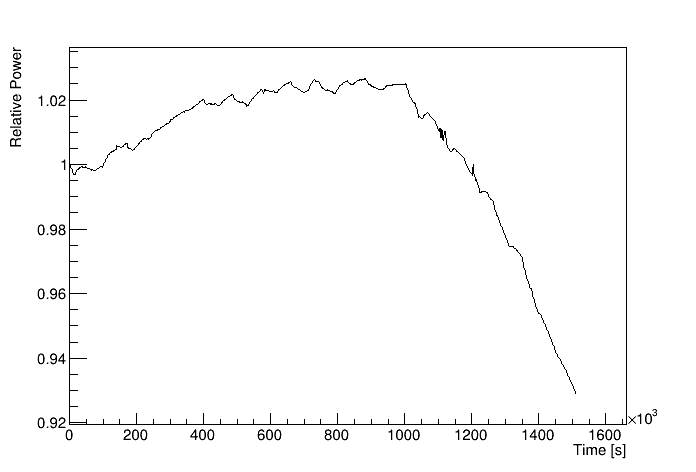
\includegraphics[scale=0.8]{./pictures/corrected1}
 \caption{Time evolution of the optical power of a single UV LED.}
 \label{SingleDiod}
\end{figure}
\par
On the Fig. \ref{SingleDiod} we can see that the optical power of single LED increased about $2 \%$ after one week. Then followed a stable interval which lasted about a week, but after that period the LED started "dying" and the power started to decrease.

\par
There are 2 mayor possibilities to fix the LED power variation problem. The first possibility is to monitor the time usage of the UV source the and according to that recalibrate the source, but the behaviour may vary diode from diode and thus it has many disadvantages. The second and more accurate approach is to regulate the power by an optical feedback.    


\subsection{Wavelength dependency}

For experiments and calibration, it is also necessary to determine the exact wavelength and its temperature dependency. We performed measurement using Ocean optics UV spectrometer along with a regulated heating plate. The LED's light was led through collimator and optical fibre directly into spectrometer's port. For every adjusted temperature, the full spectral profile of the UV LED is measured. Both the heating plate and the spectrometer are controlled by the RPi. The main part of spectral data is fitted with a gaussian and its parameters are used to obtain wanted physical quantities: $\mu$ - the main wavelength $\lambda$, $\sigma$ - the wavelength interval $\Delta \lambda$. The uncertainties are taken from the fit.


\begin{figure}[H]
 \centering
 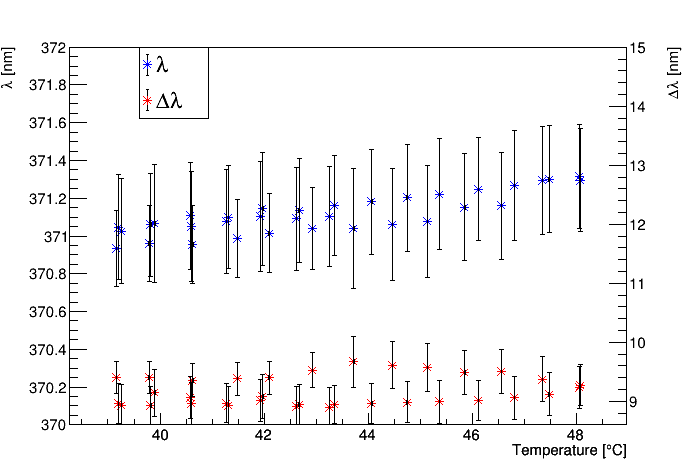
\includegraphics[scale=0.65]{./pictures/SpectreShakeWave}
 \caption{$\lambda$ and $\Delta \lambda$ temperature dependency.}
 \label{wavdep}
\end{figure}

On the Fig. \ref{wavdep} we can see, that both $\lambda$ and $\Delta \lambda$ dependencies on temperature are insignificant.

%------------------------------------------------
\section{Optical feedback - potential fix}
% -----------------------------------------------
One way to handle the ageing process of UV LED diodes is to monitor the power and according to the changes set the diode current $I_\textrm{d}$. To achieve that, we tried to develop a prototype of optical feedback concept, which is based on detection UV photodiode. 
\par
The part of optical power is reflected from LED to photodiode. Photocurrent induced this way is converted to voltage which is read by ADC (analog-digital converter). This information is then used by the STM32 board to adjust the current level by DAC. One problem is that the optical power is delivered in pulses, and thus it is necessary to sample these pulses and determine the height.
\par
\subsection{Detection photodiode}
As detection photodiode we chose GUVV-T10GD (or GUVV-C20SD as SMD equivalent). It is guaranteed to be UV-A sensor with wavelength responsivity from 230 to 395 nm. However, it is necessary to test more of its properties, because some of the properties, which are essential for our application, are not shown in datasheets and probably haven't been yet measured - temperature dependency of the dark current, responsivity to 10 $\mu$s square signals and ageing processes. The reverse voltage of photodiode $U_\textrm{r}$ could go up to 2 V. With higher the $U_\textrm{r}$ is, the lower is the diode's capacity.
\par
\subsubsection{Dark current}
Information of dark current is very important. We need to know if the signal levels are much greater than dark current. We measured dark current with 7 set temperatures. Current was measured by Keithley 2470 picoammeter. Temperature was set by autoregulated transistor heating plate. The transistor plate is driven by STM32 nucleo's DAC. The nucleo is controlled by the RPi. The RPi also communicates with picoammeter and controls the entire data acquisition. We measured two series - one with reverse voltage $U_\textrm{r} = 0.1$ V and second with reverse voltage $U_\textrm{r} = 1$ V. The picoammeter is also capable of providing voltage, so it was used as a source of reverse voltage.

\begin{figure}[H]
 \centering
 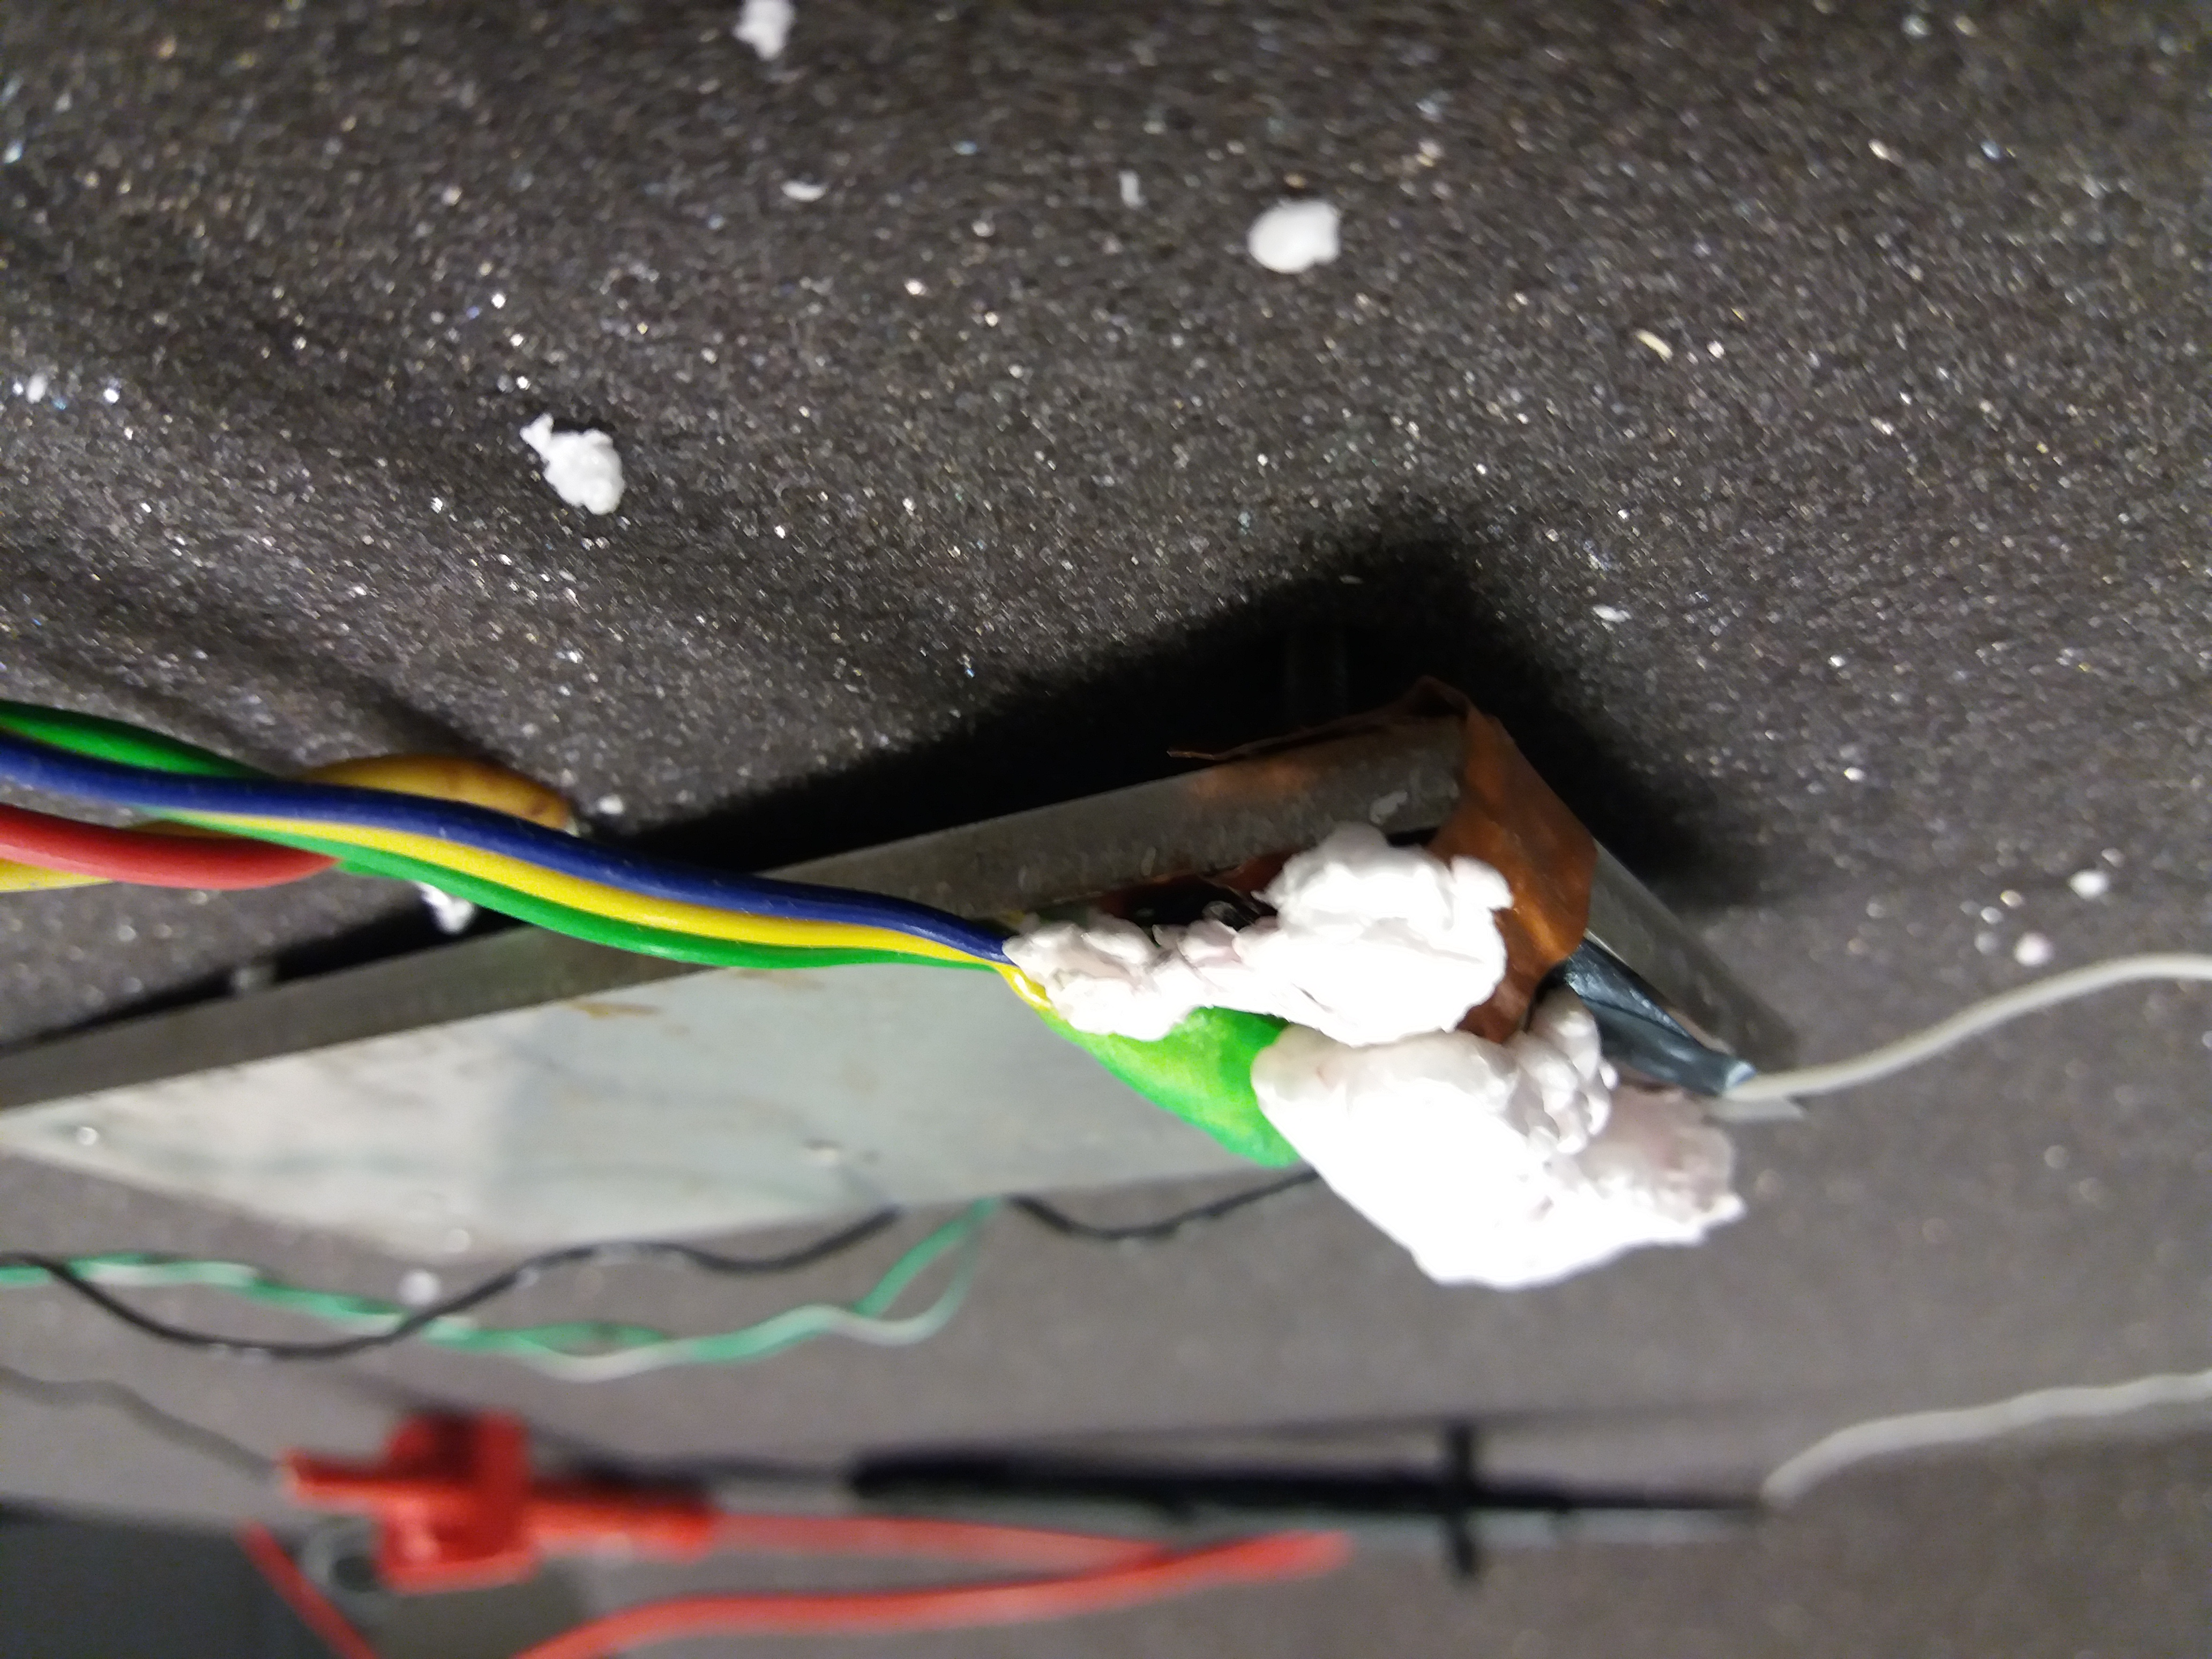
\includegraphics[scale=0.09, angle = 180]{./pictures/DiodeHeat}
 \caption{UV detection diode mounted on heating plate, covered by insulating material. The thermometer is mounted next to it.}
 \label{heatDiode}
\end{figure}


\begin{figure}[H]
 \centering
 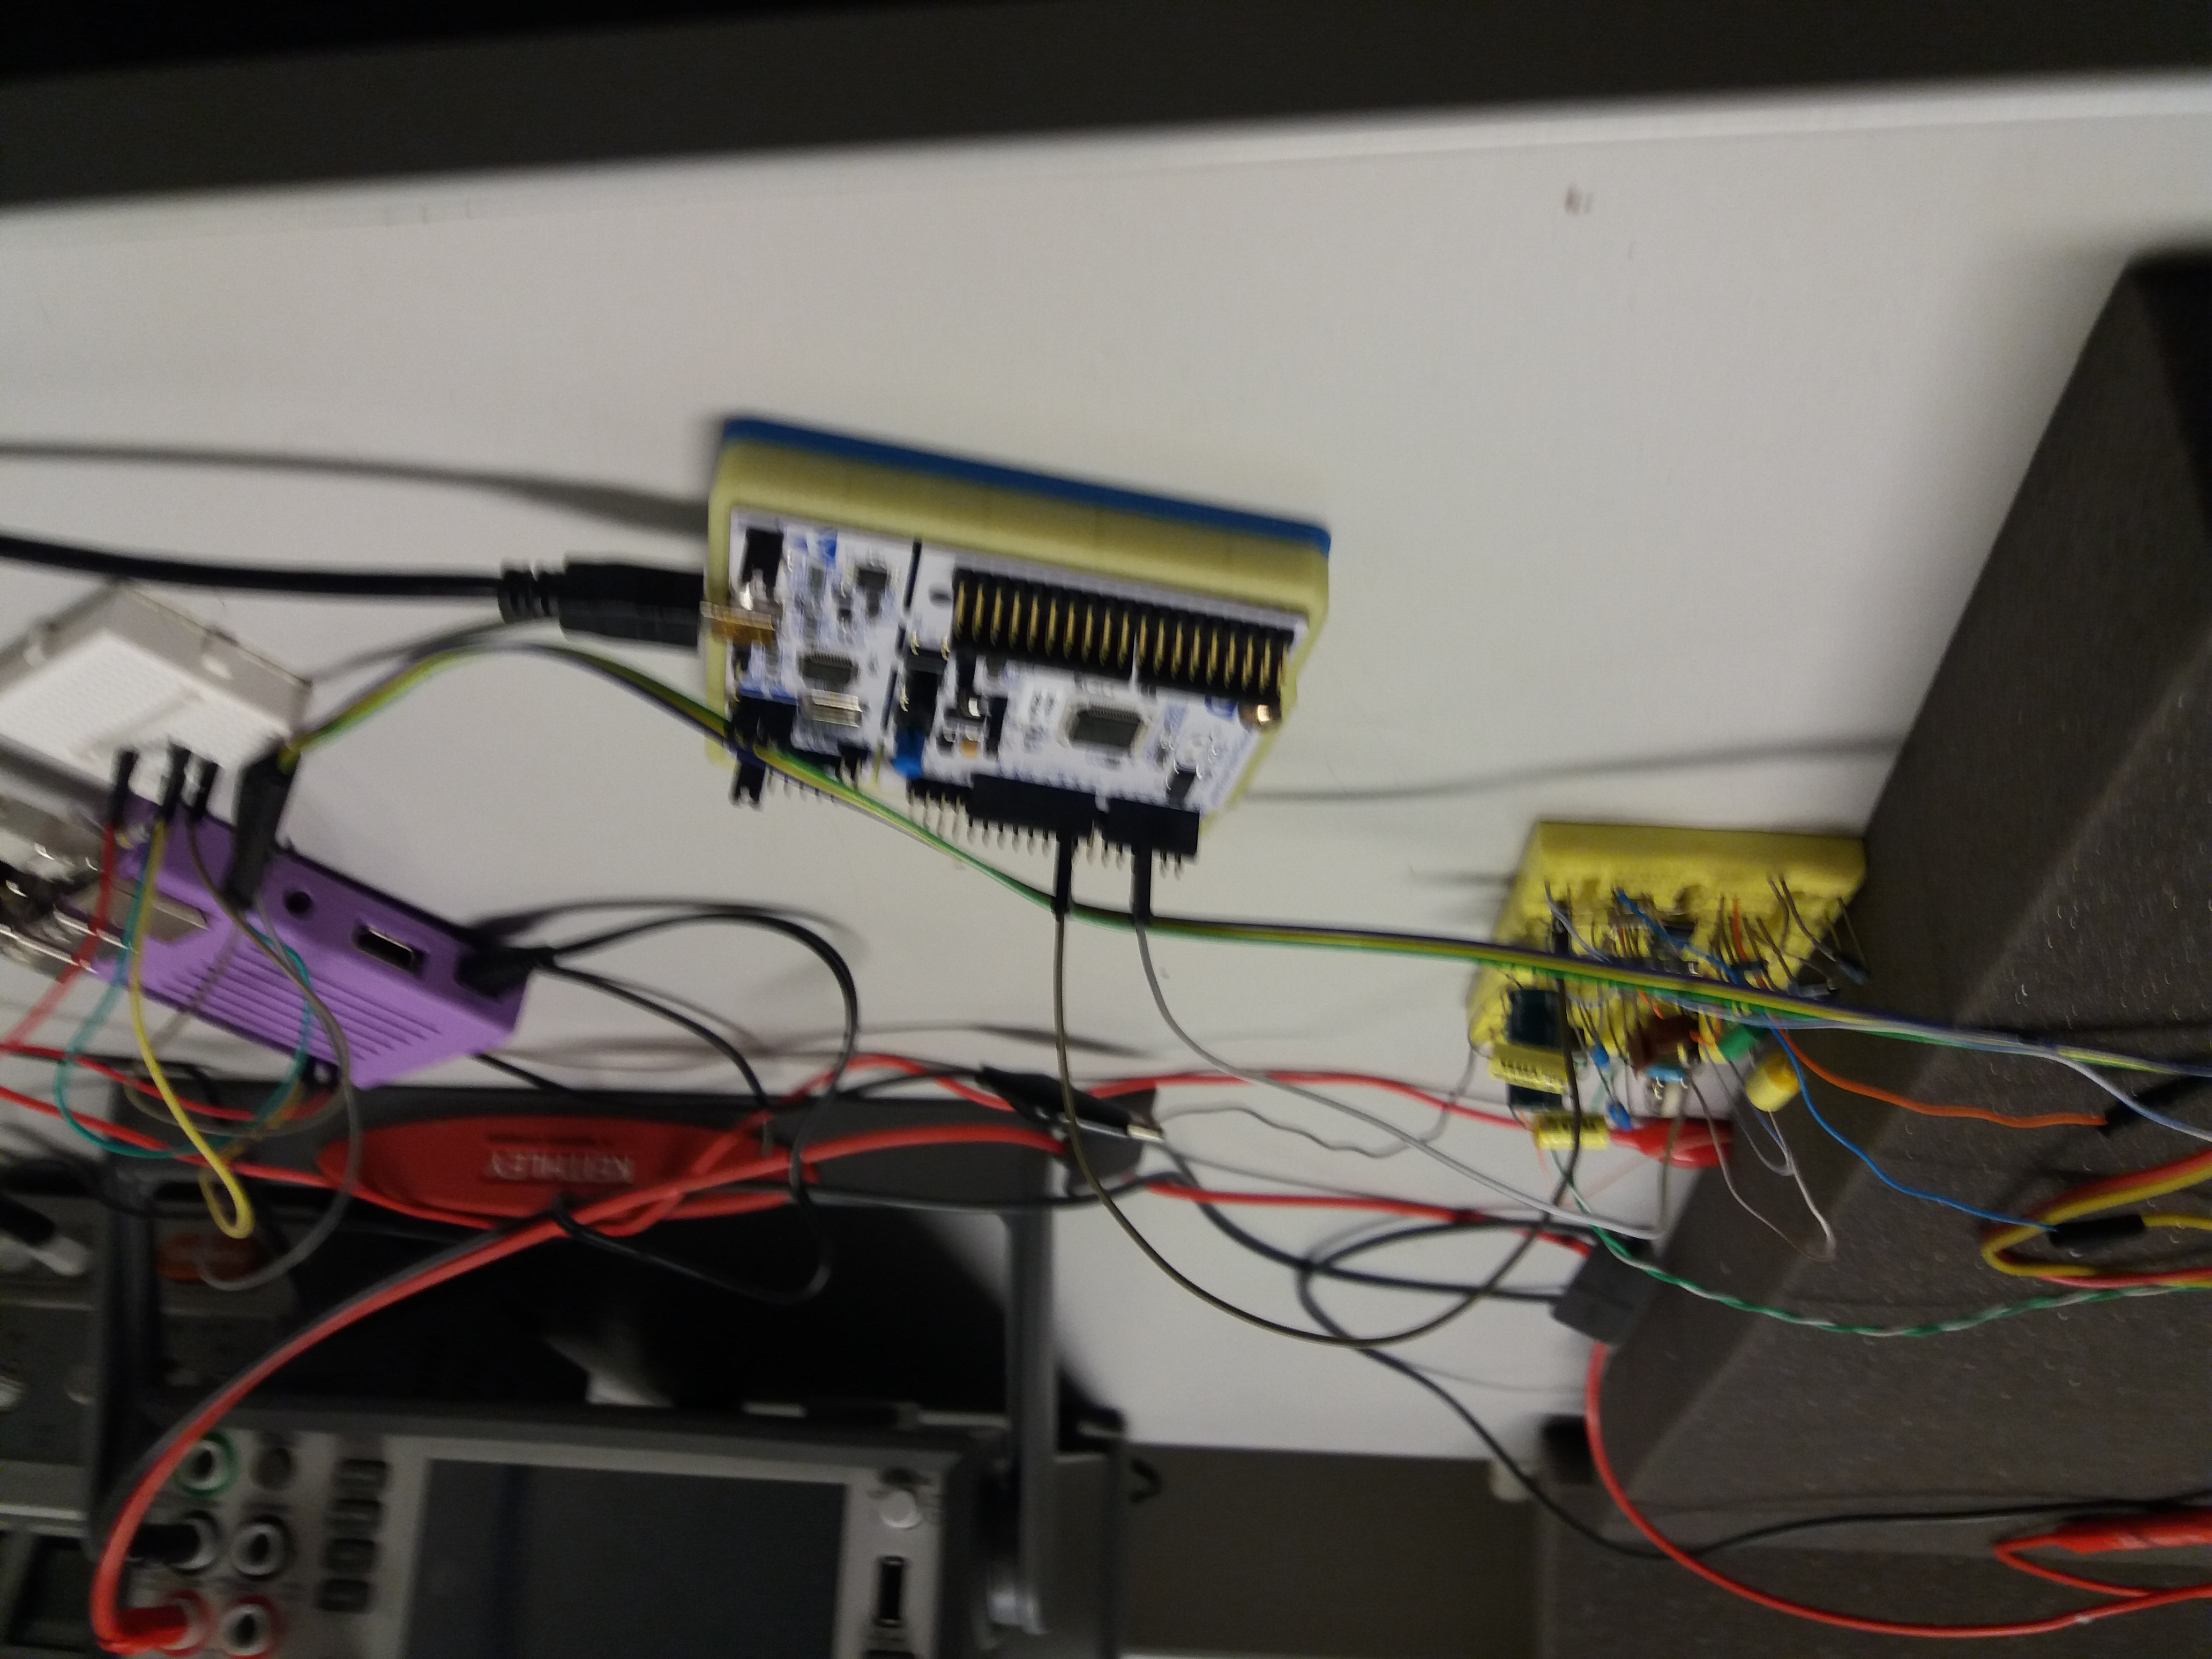
\includegraphics[scale=0.09, angle = 180]{./pictures/heating}
 \caption{Heating control and measurement control. From the left - heating circuit, STM32 nucleo, RPi}
 \label{heating}
\end{figure}



\begin{figure}[H]
 \centering
 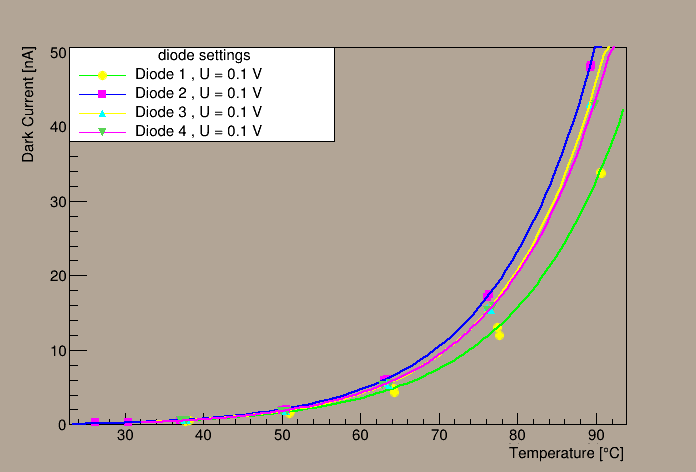
\includegraphics[scale=0.8]{./pictures/01V}
 \caption{Dark currents with the reverse voltage $U_\textrm{r}= 0.1$ V.}
 \label{01V}
\end{figure}

\begin{figure}[H]
 \centering
 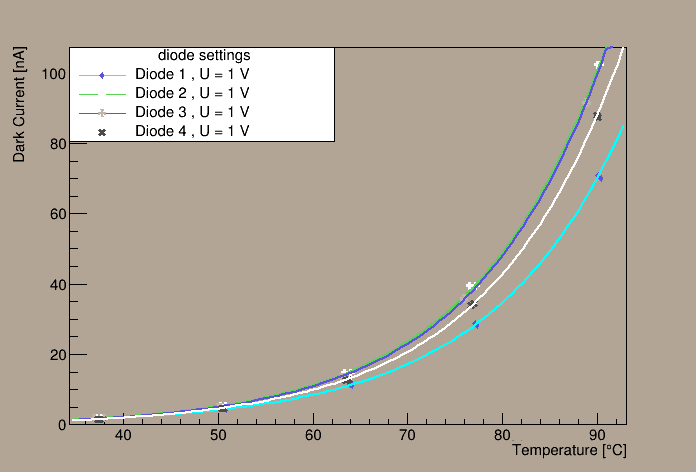
\includegraphics[scale=0.8]{./pictures/1V}
 \caption{Dark currents with the reverse voltage $U_\textrm{r}= 1$ V.}
 \label{1V}
\end{figure}


We measured 5 diodes. However, the dark currents of one diode were on abnormal level, and that's why its characteristics are not plot in graphs with others. This diode was not suitable for our application.
\par

From the measured data we can see, that for the expected operating temperatures ($t < 50^{\circ}C$), the dark current is $I_{dark} < 10$ nA. 

\subsubsection{Signal responsivity}
By direct illumination of the photodiode by the UV LED ($I_d = 7.5 $ mA) we are able to induce photocurrent about $I_\textrm{p} = 5$ $\mu$A, which is of the higher order than the measured dark current.
\par
To test responsibility of the square pulses, we integrated the photodiode into the $I/U$ trans-impedance amplifier with the op-amp ADA4805 with feedback parameters $R_\textrm{F} = 100$ k$\Omega$ and $C = 9$ pF. We illuminated the photodiode by the UV LED connected to the square pulse generator. The response could be seen on Fig. \ref{response}.

\begin{figure}[H]
 \centering
 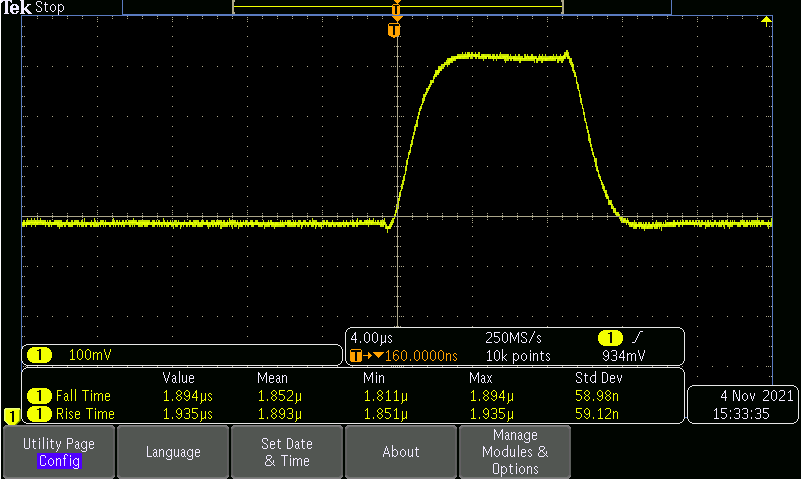
\includegraphics[scale=0.5]{./pictures/pulse}
 \caption{Photodiode's response on 10 $\mu$s square pulse.}
 \label{response}
\end{figure}


This way we are able to see the pulsing UV LED light. However, the rising edge of feedback pulse is deformed. 

\subsubsection{Artificial ageing}
For the feedback photodiode, the time stability is very important. It has to last much more than the LED. To test the long-time stability, we tried to artificially age the feedback photodiode. It is well-known fact from the molecular physics, that the diffusion coefficients of most materials depends on temperature and they grow with increasing temperature \cite{Diff}. So we tried to speed up the ageing by holding the photodiode just under the maximum of operating temperature (on $80^{\circ}$C) for one week. During that period, the photodiode was illuminated by UV LED and the photocurrent was measured (Fig. \ref{agingPhotoCurrent}).


\begin{figure}[H]
 \centering
 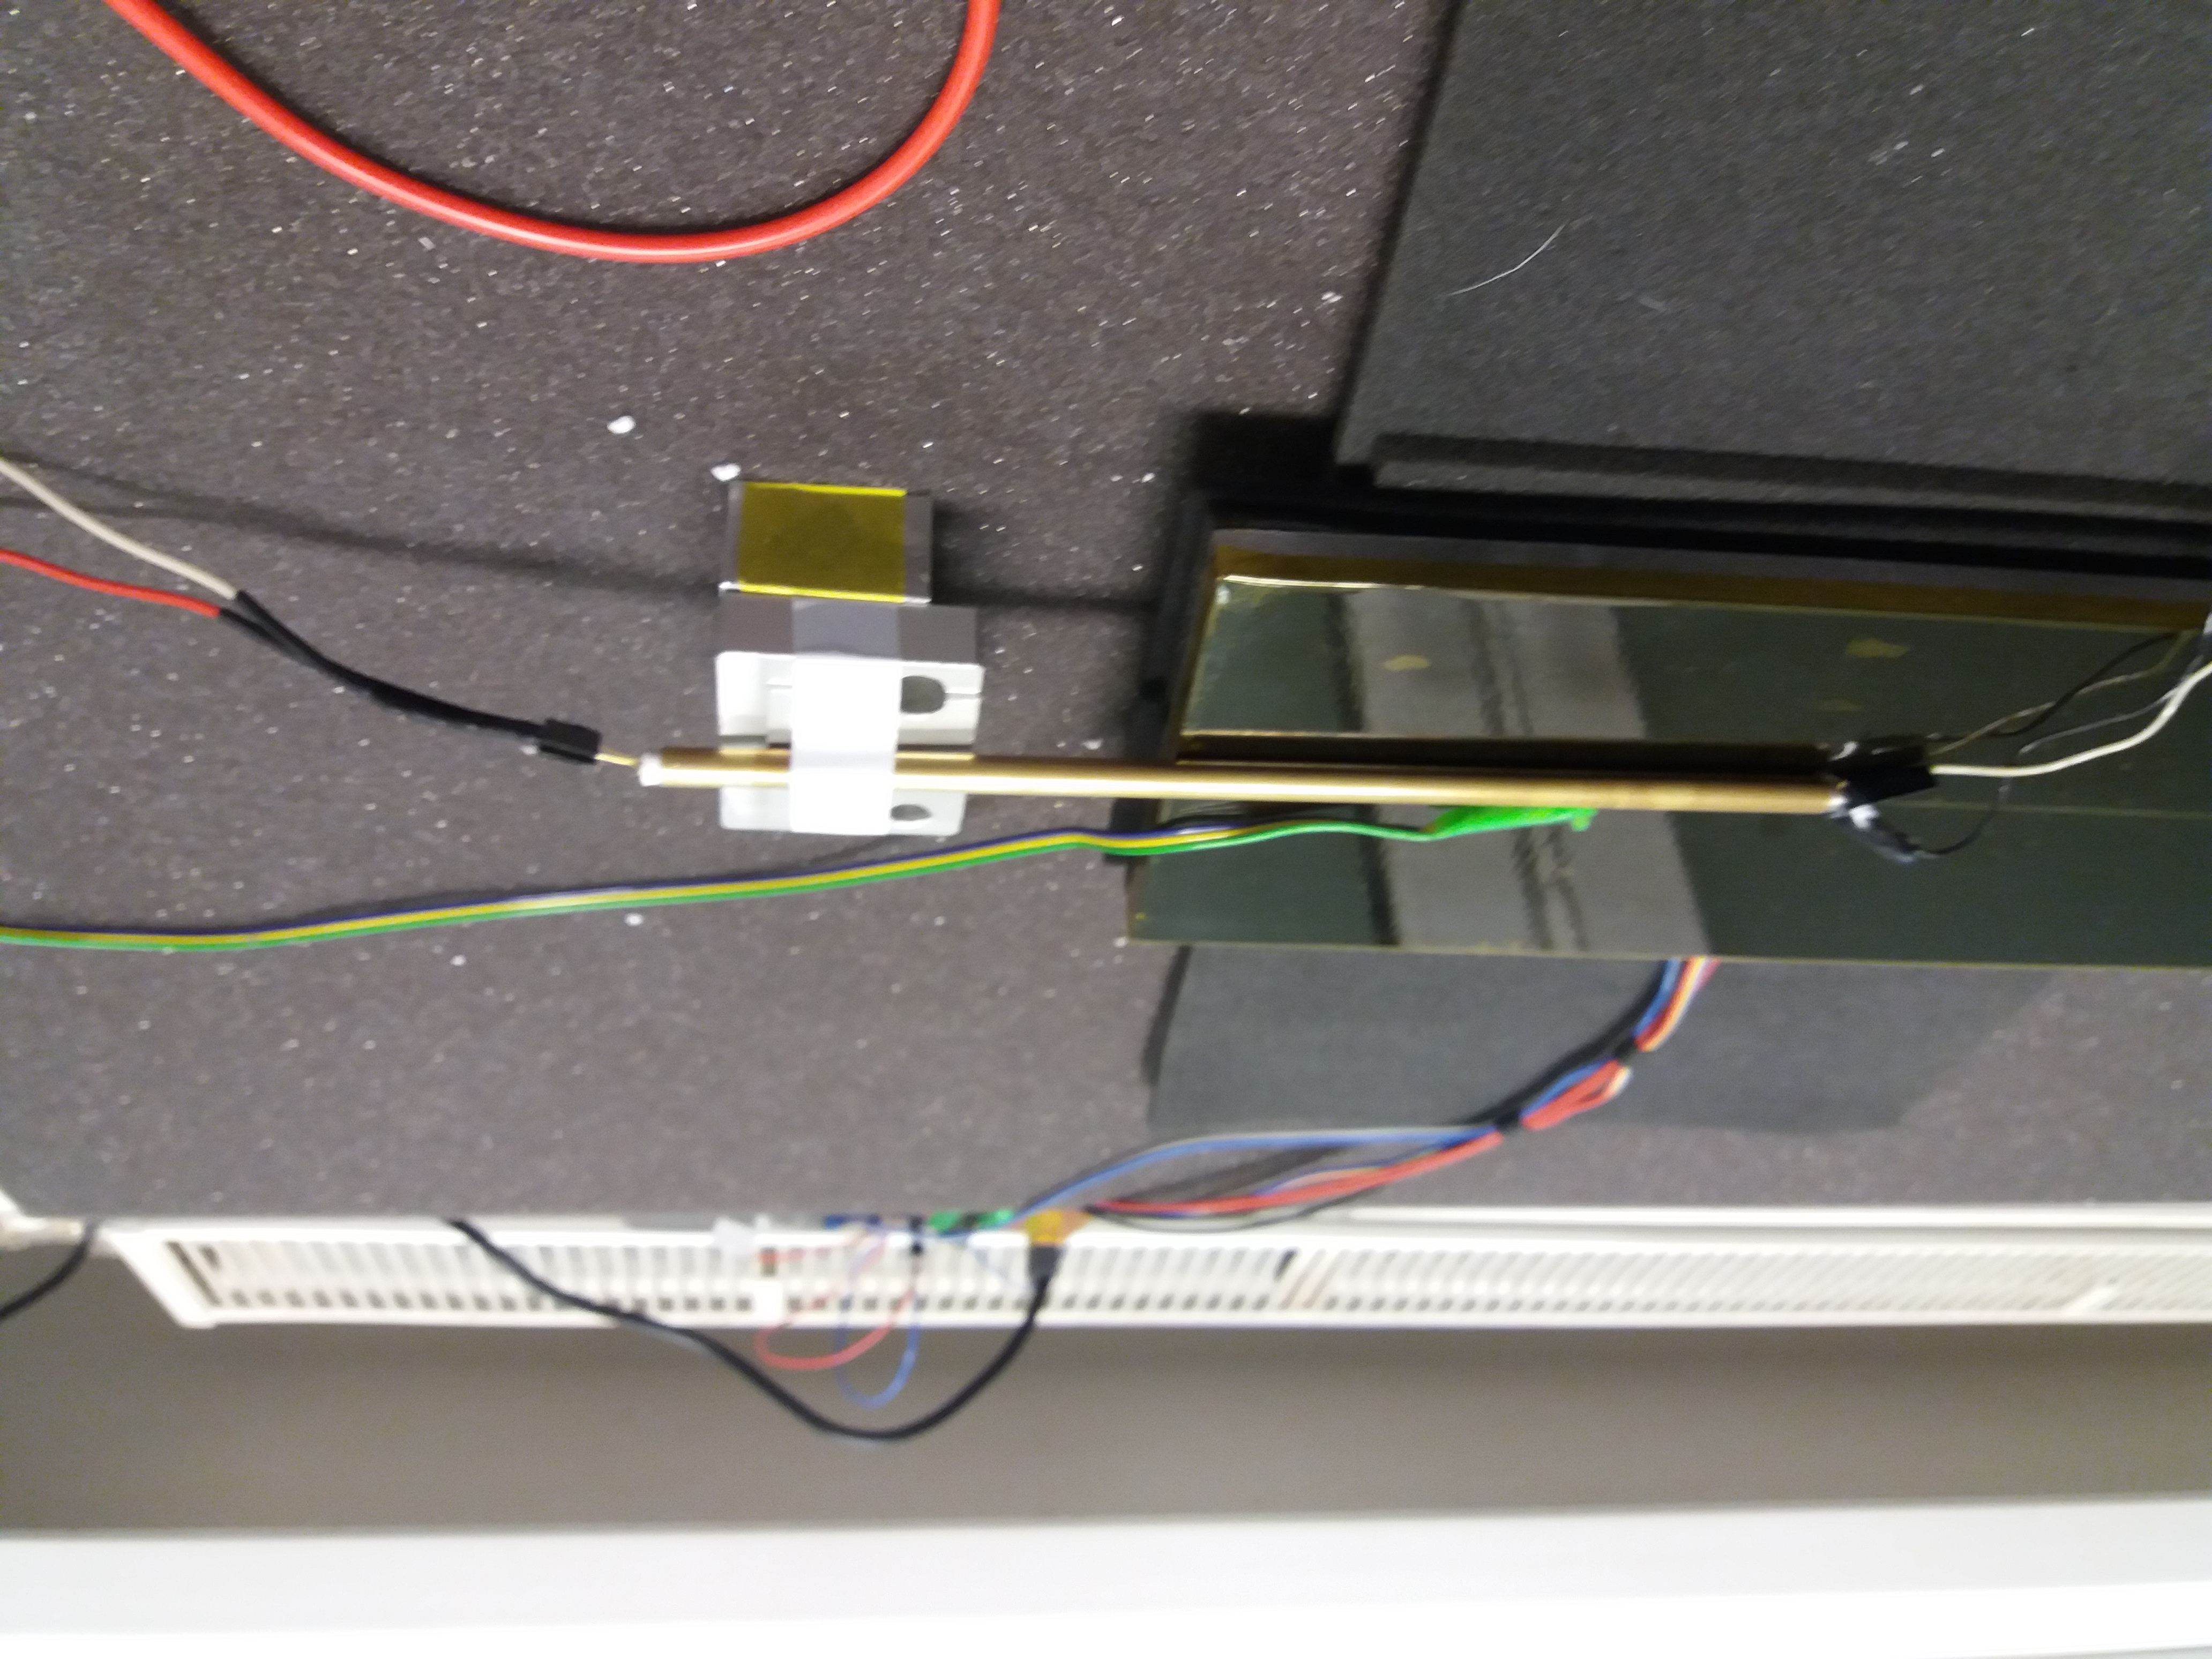
\includegraphics[scale=0.08, angle=180]{./pictures/TempDestrc}
 \caption{Photodiode mounted on bigger transistor heating and illuminated by LED through pipe.}
 \label{aging}
\end{figure}


\begin{figure}[H]
 \centering
 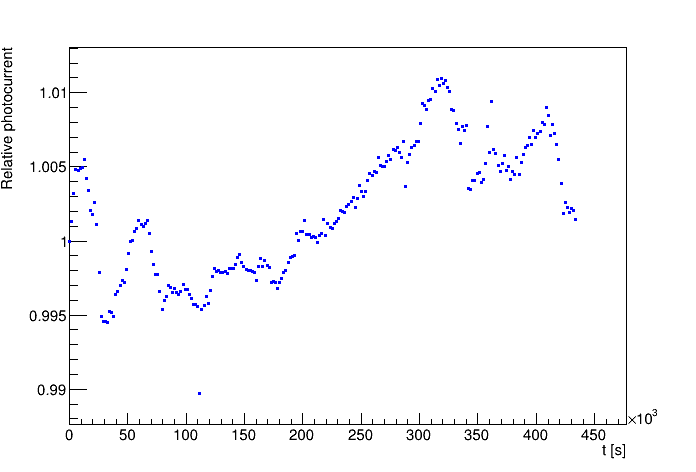
\includegraphics[scale=0.6]{./pictures/ArtiAging}
 \caption{Time evolution of the photodiode's photocurrent.}
 \label{agingPhotoCurrent}
\end{figure}

The time evolution shows that the photodiode's photocurrent increased around 1 $\%$ over one week. However, this small variation is probably caused by the LED ageing, as was shown before. 
\par
Due to the fact, that any bigger drift in sensitivity was not observed under the bad conditions, we come to a conclusion that the feedback photodiode is much more stable than the LED.

\subsection{Feedback concept and testing}

The original concept circuit was modified by adding the feedback part, which consists of two op amps - primary acts as trans-impedance amplifier (LTC6268) to convert induced photocurrent into the signal voltage and the secondary acts as a simple voltage amplifier/follower (ADA4805) with pre-filter. The photodiode is powered by a voltage regulator (LT1054). The additional scheme can be seen on Fig. \ref{Amplifier}.
   
\begin{figure}[H]
 \centering
 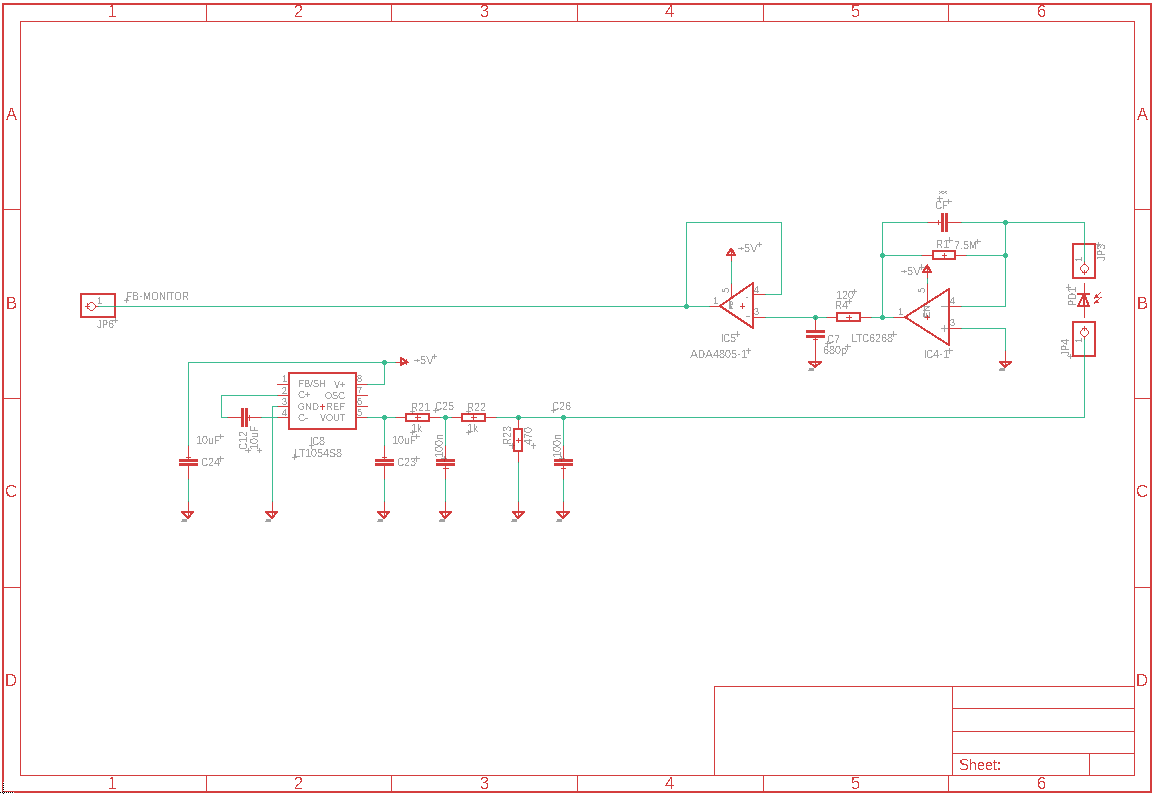
\includegraphics[scale=0.45]{./pictures/FeedBackCirc.png}
 \caption{Two state amplifier with a photodiode scheme. Physically manufactured by Vladimír Urbášek.}
 \label{Amplifier}
\end{figure}

The UV LED is mounted in position to deliver power into the photodiode and also to an output port. The optomechanical system can be seen on Fig. \ref{Optomechanics}. The prototype consists of two circuits - of the LED driver and the feedback detector, bound together by 3D printed parts.

\begin{figure}[H]
 \centering
 \includegraphics[scale=0.09]{./pictures/optomechanics.png}
 \caption{Optomechanics with a feedback illustration.}
 \label{Optomechanics}
\end{figure}


However, the UV source is designed to deliver 10$\mu$s pulses, so, to determine the signal level, it is necessary to sample this pulse. 

\subsubsection{Sampling and regulation}

To perform the pulse sampling, the hardware with enough capabilities has to be used. STM32 board Nucleo F446RE \cite{NucF446RE} offers various timers (for PWM generation and advanced triggering), both 12-bit ADC and DAC and a DMA (direct memory access) feature. The ADC combined with DMA can flush the sampled data directly into the memory and may exceed the sample rate over 1 MS/s.

\par

The other problem is the time synchronization of sampling with the pulse, to achieve that the STM32 timers have to be combined. Due to the fact, that the excitation PWM pulses for the LED circuit are generated by STM32 timer, there is a possibility to use this PWM timer also to trigger an another timer (programmed as a slave), which can handle the ADC sampling. Some timers can be programmed to produce a burst of short pulses with defined number of repeats. These short pulses can be used to trigger ADC to take sample and transfer it directly into memory through DMA without any necessity of the CPU handling.  
\par
The sampling procedure captured by oscilloscope can be seen on Fig. \ref{procedure}. Blue is the original PWM excitation pulse for LED current driver, yellow is the optical pulse captured by photodiode, and violet are the pulses generated by the slave timer triggering the ADC samples. Due to the deformation of the yellow photodiode signal, the first two samples are not taken to account. 
There may be a space for two more samples to be taken at the end of the yellow pulse, but we decided not to do so, because of the possible prototyping variations in the pulse's end edge. 


\begin{figure}[H]
 \centering
 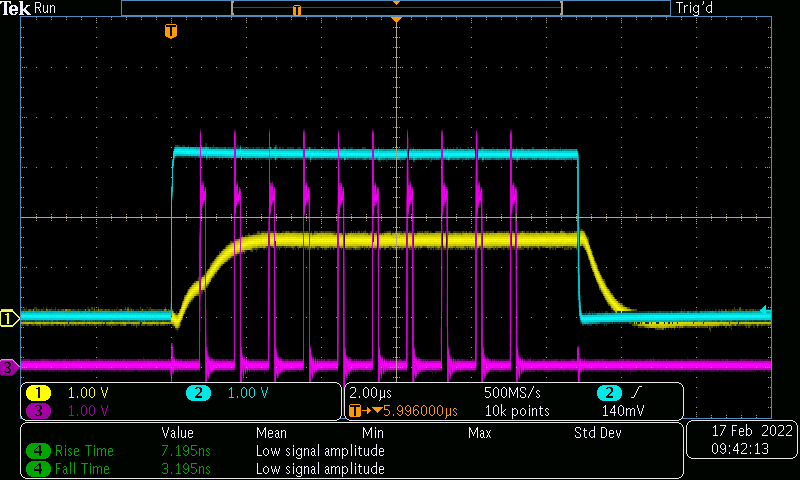
\includegraphics[scale=0.5]{./pictures/PWMSampling.png}
 \caption{Pulse sampling procedure captured by oscilloscope. Blue - original PWM excitation pulse, yellow - optical pulse captured by photodiode, and violet - pulses generated by the slave timer triggering the ADC samples.}
 \label{procedure}
\end{figure}
\par
This synchronized sampling can produce up to 8 samples per pulse. To achieve better statistics, we decided to capture and sample about 50 pulses. The mean value of these samples is considered to be a level of the actual LED power. This value is then used by STM32's program to set the DAC value. However, the direct setting of DAC by actual value of LED power is not suitable for this application and may cause unwanted oscillations in power level, and thus it is better to implement some kind of numerical regulation.


\par
In many applications it is needed to dynamically vary the output to compensate unwanted effects the and to achieve the stability of some physical quantity (temperature, position etc.). The most basic approach is the PID regulation (proportional-integral-derivative). PID regulation is based on a feedback loop - the error value is calculated from the difference of a current measured state and a desired state. Output is then set to the value calculated as a weighted sum proportional, integral and derivative terms of the error value (both integral and derivative are numerically calculated). This is repeated in cycle, with recalculating error value and its terms \cite{PID}. The new value for DAC is set in every cycle.

\par
For our purposes, where the output state (optical power) is set by DAC, the regulation based only on the integral term was implemented. This concept allows optical power to rapidly increase when it is too far from desired value and also to make fine corrections when the optical power starts to deviate from the desired value. 

\par

The original ADC and DAC reference is 3.3 V made from the supply voltage stabilizer, which does not have the required accuracy and may vary with the supply voltage. For the feedback purposes the STM32 reference pin was reconnected to the external, more accurate 2V reference along with a 50nF capacitor to prevent board's internal oscillators from jamming the reference stability.     




\subsubsection{Direct stabilization test}

Before running any long-time tests, the stabilization has to be simply tested, for example by varying the transmission between the two diodes.
\par
To vary the transmission, and thus to simulate the optical power variations, inserting a simple paper shade directly into the optomechanics between the two diodes has proven to be enough for this experiment.

\begin{figure}[H]
 \centering
 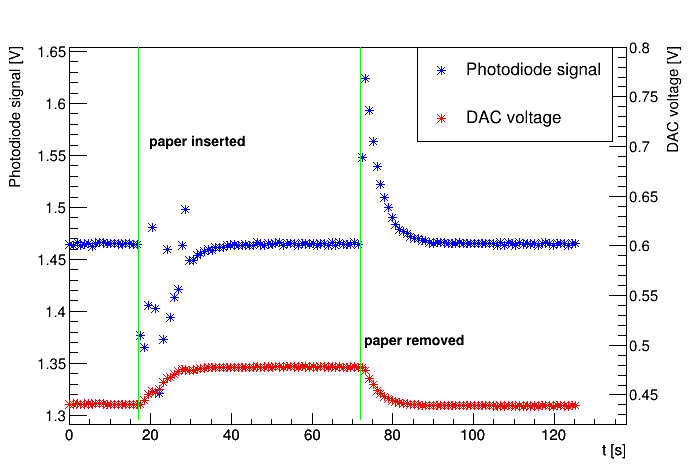
\includegraphics[scale=0.5]{./pictures/Stabilizin.png}
 \caption{Feedback concept testing.}
 \label{Feedback testing}
\end{figure}

From the Fig. \ref{Feedback testing} we can see, that after the paper is inserted, the photodiode signal rapidly decreases, but the feedback detects this and begins to increase the DAC voltage (and thus the LED current) until the photodiode signal reaches the same value as it had before the transmission was altered. After removing the paper, the LED power is high, so the photodiode signal jumps onto the high level too. The feedback detects this again and lowers the DAC voltage to the original value. 
\par
This behaviour is what was expected. However, the long-time test similar to the previous tests of the original UV source has to be performed either way. 


\subsubsection{Long-time test}

Due to the non-optimized optomechanics the source was not able to produce enough light for the test in the IS, so the power meter was mounted directly onto the output of the prototype. Also the pre-testing has shown that the prototype is incapable to fully compensate the temperature variations. The most probable cause of these temperature variations is the thermal expansion of the mechanics. Many of the other possible causes (LED spectral dependency, voltage reference stability etc.) were tested without having any impact on the prototype's behaviour. 


\par
The test run was done on heating plate having both the prototype and Nucleo stabilized on $t \approx 40.5$ $^\circ $C (the heating itself is incapable of holding the temperature with accuracy better than 1 $^\circ $C) and covered by an insulating material. Besides the optical power measurement, the DAC value (voltage - measured by multimeter) was also measured to observe the feedback stabilization. To measure optical power with the power meter, the pulse's duty cycle was increased to 50 $\%$, but the sampling scheme was unchanged.

\par

The test lasted about 10 days and the results can be seen on Fig. \ref{Long test}.


\begin{figure}[H]
 \centering
 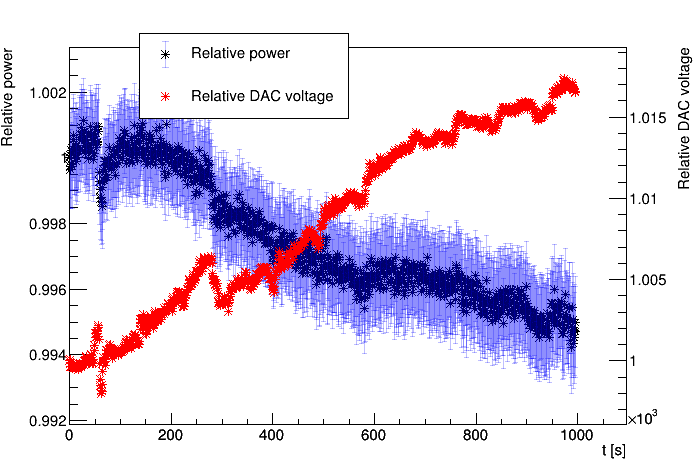
\includegraphics[scale=0.5]{./pictures/LongTime.png}
 \caption{Long time test of the feedback UV source prototype.}
 \label{Long test}
\end{figure}

\begin{figure}[H]
 \centering
 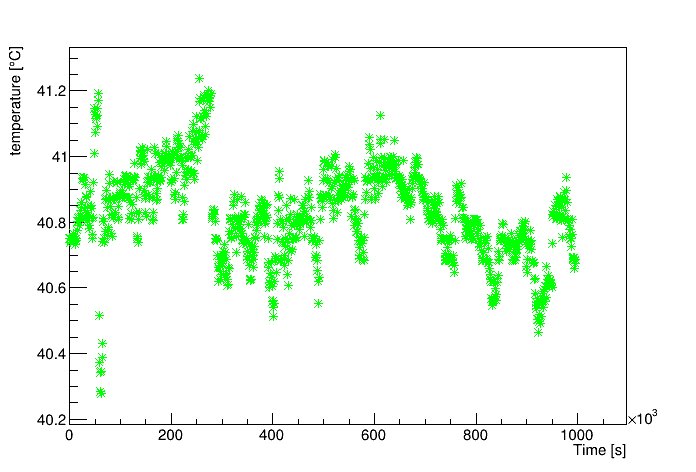
\includegraphics[scale=0.5]{./pictures/LastTemp.png}
 \caption{Temperature of the heating plate evolution.}
 \label{Long test temperatures}
\end{figure}

From the relative optical power time evolution we can see, that it decreased about 0.005 $\%$ in 10 days. This change can be partially associated with temperature drop about 0.2 $^\circ$C from Fig. \ref{Long test temperatures}. However, the DAC value increased about 1.7 $\%$ and it is highly possible, that this was the way the feedback loop balanced the LED's power decrease.

\par 
 
Although there was a 0.005 $\%$ change in optical power, this test can be considered to be the most sufficient test of the UV source stability so far. However, the UV source prototype is not yet ready to fully serve the FAST's calibration procedures. There is yet much to be done - temperature stabilization, fine mechanics and user-friendly control.


%------------------------------------------------
% -----------------------------------------------



% -----------------------------------------------
% %%%%%%%%%%%%%%%%%%%%%%%% End of file %%%%%%%%%%%%%%%%%%%%%%%%

% -----------------------------------------------
% Závěr
% -----------------------------------------------
\chapter*{Conclusion}
\addcontentsline{toc}{chapter}{Conclusion}

We are completely f****d.

% -----------------------------------------------
% Literatura a prameny
% -----------------------------------------------
%\begin{thebibliography}{99}
\bibliographystyle{apsrev4-2}
\nocite{*}
\bibliography{citations}
%\addcontentsline{toc}{chapter}{Literatura}
%\bibitem{gravitation} MISNER, Ch. W.; THORNE, K. S.; WHEELER, J. A. %\emph{Gravitation}. San Francisco: W. Freeman, 1973.
%\end{thebibliography}

\newpage
Preferované jsou citace podle norem ČSN ISO 690 a ISO 690-2, popř. styly APS (American Physical Society – u~prací zaměřených fyzikálně) nebo APA (American Psychological Association – u~prací zaměřených více didakticky a pedagogicky).
\end{document}
% Konec souboru %%%%%%%%%%%%%%%%%%%%%%%%%%%%%%%%%%%%%%%%%%%%%%%%%%%%%%%%%%%%
